\section{Observations}

According the \ref{se:test_plan} section, this section includes the observations after performing the test plans on the \acrshort{wdias} system setup and test plan test up which is explained in the \ref{se:workload}.

Sections \ref{subse:obs_test_plan_all_60min} to \ref{subse:obs_test_plan_all_auto_15min} discuss the observations collected with performing the Load test plans over 60 minutes (24 data points), 30 minutes (48 data points) and 15 minutes (96 data points) by variate the request size. Then another performance test with enabling Auto Scaling as explained in \ref{subse:test_plan_metrics} for high resource utilized microservice.

%%%%%%%%%%%%%%%%%%%%%%%%%%%%%%%%%%%%%%%%%%%%%%%%%%%%%%%%%%%%%%%%%%%%%%%%%%%%%%%%
\subsection{Load Testing with hourly data (24 Request Size)}
\label{subse:obs_test_plan_all_60min}

After running the All test plan with 60 minutes (24 data points), it observed the data summary of \ref{tab:obs_all_60_min_summary}. It performed 311k of sample requests.

\begin{table}[ht]
\caption{Throughput and Latency of load testing with 60min data}
\footnotesize
\begin{tabulary}{\linewidth}{|L|C|C|C|C|C|C|C|C|}
\hline
Label & \# Samples & Avg & Min & Max & 90\% Line & Std. Dev. & Error \% & RPS \\ \hline
Insert Timeseries & 71826 & 28 & 13 & 2773 & 31 & 58.74 & 0.00\% & 40.5 \\ \hline
Retrieve Timeseries & 71796 & 8 & 7 & 242 & 10 & 4.18 & 0.00\% & 40.7 \\ \hline
Insert Grid & 7982 & 23 & 21 & 126 & 26 & 4.23 & 0.06\% & 4.5 \\ \hline
Retrieve Grid & 7979 & 68 & 59 & 238 & 75 & 10.11 & 0.00\% & 4.5 \\ \hline
Query: Location & 71804 & 3 & 2 & 109 & 3 & 1.52 & 0.00\% & 40.5 \\ \hline
\textbf{TOTAL} & 311182 & 127 & 0 & 2773 & 503 & 207.80 & 0.00\% & 175.4 \\ \hline
\end{tabulary}
\label{tab:obs_all_60_min_summary}
\end{table}
Insert Timeseries performed over Scalar and Vector data types with each request send with 24 data points. On average it takes 28ms to insert data into the \acrshort{wdias}, and up to 90\% percentile inserted data within 31ms. Noticeably it has 0\% of errors which means that all the request are completed successfully. On average, \acrshort{wdias} handled 40.5 \acrshort{rps} with the given workload. The performance of the Retrieve of Scalar and Vector Timeseries are similar to insert timeseries due to it depends on it.
On the other hand, Insert Grid Timeseries data perform with 23ms with almost all the request perform within same amount of time, hence the standard deviation is smaller. Retrieve Grid Timeseries data perform the same but with bit higher value of latency of 68ms. Both of insert and retrieve grid timeseries data have 4.5 \acrshort{rps} since it only get 10\% of the number of request per given time via the test plan as explain in the data ration in \ref{se:test_plan}.

\begin{figure}[htp]
    \centering
    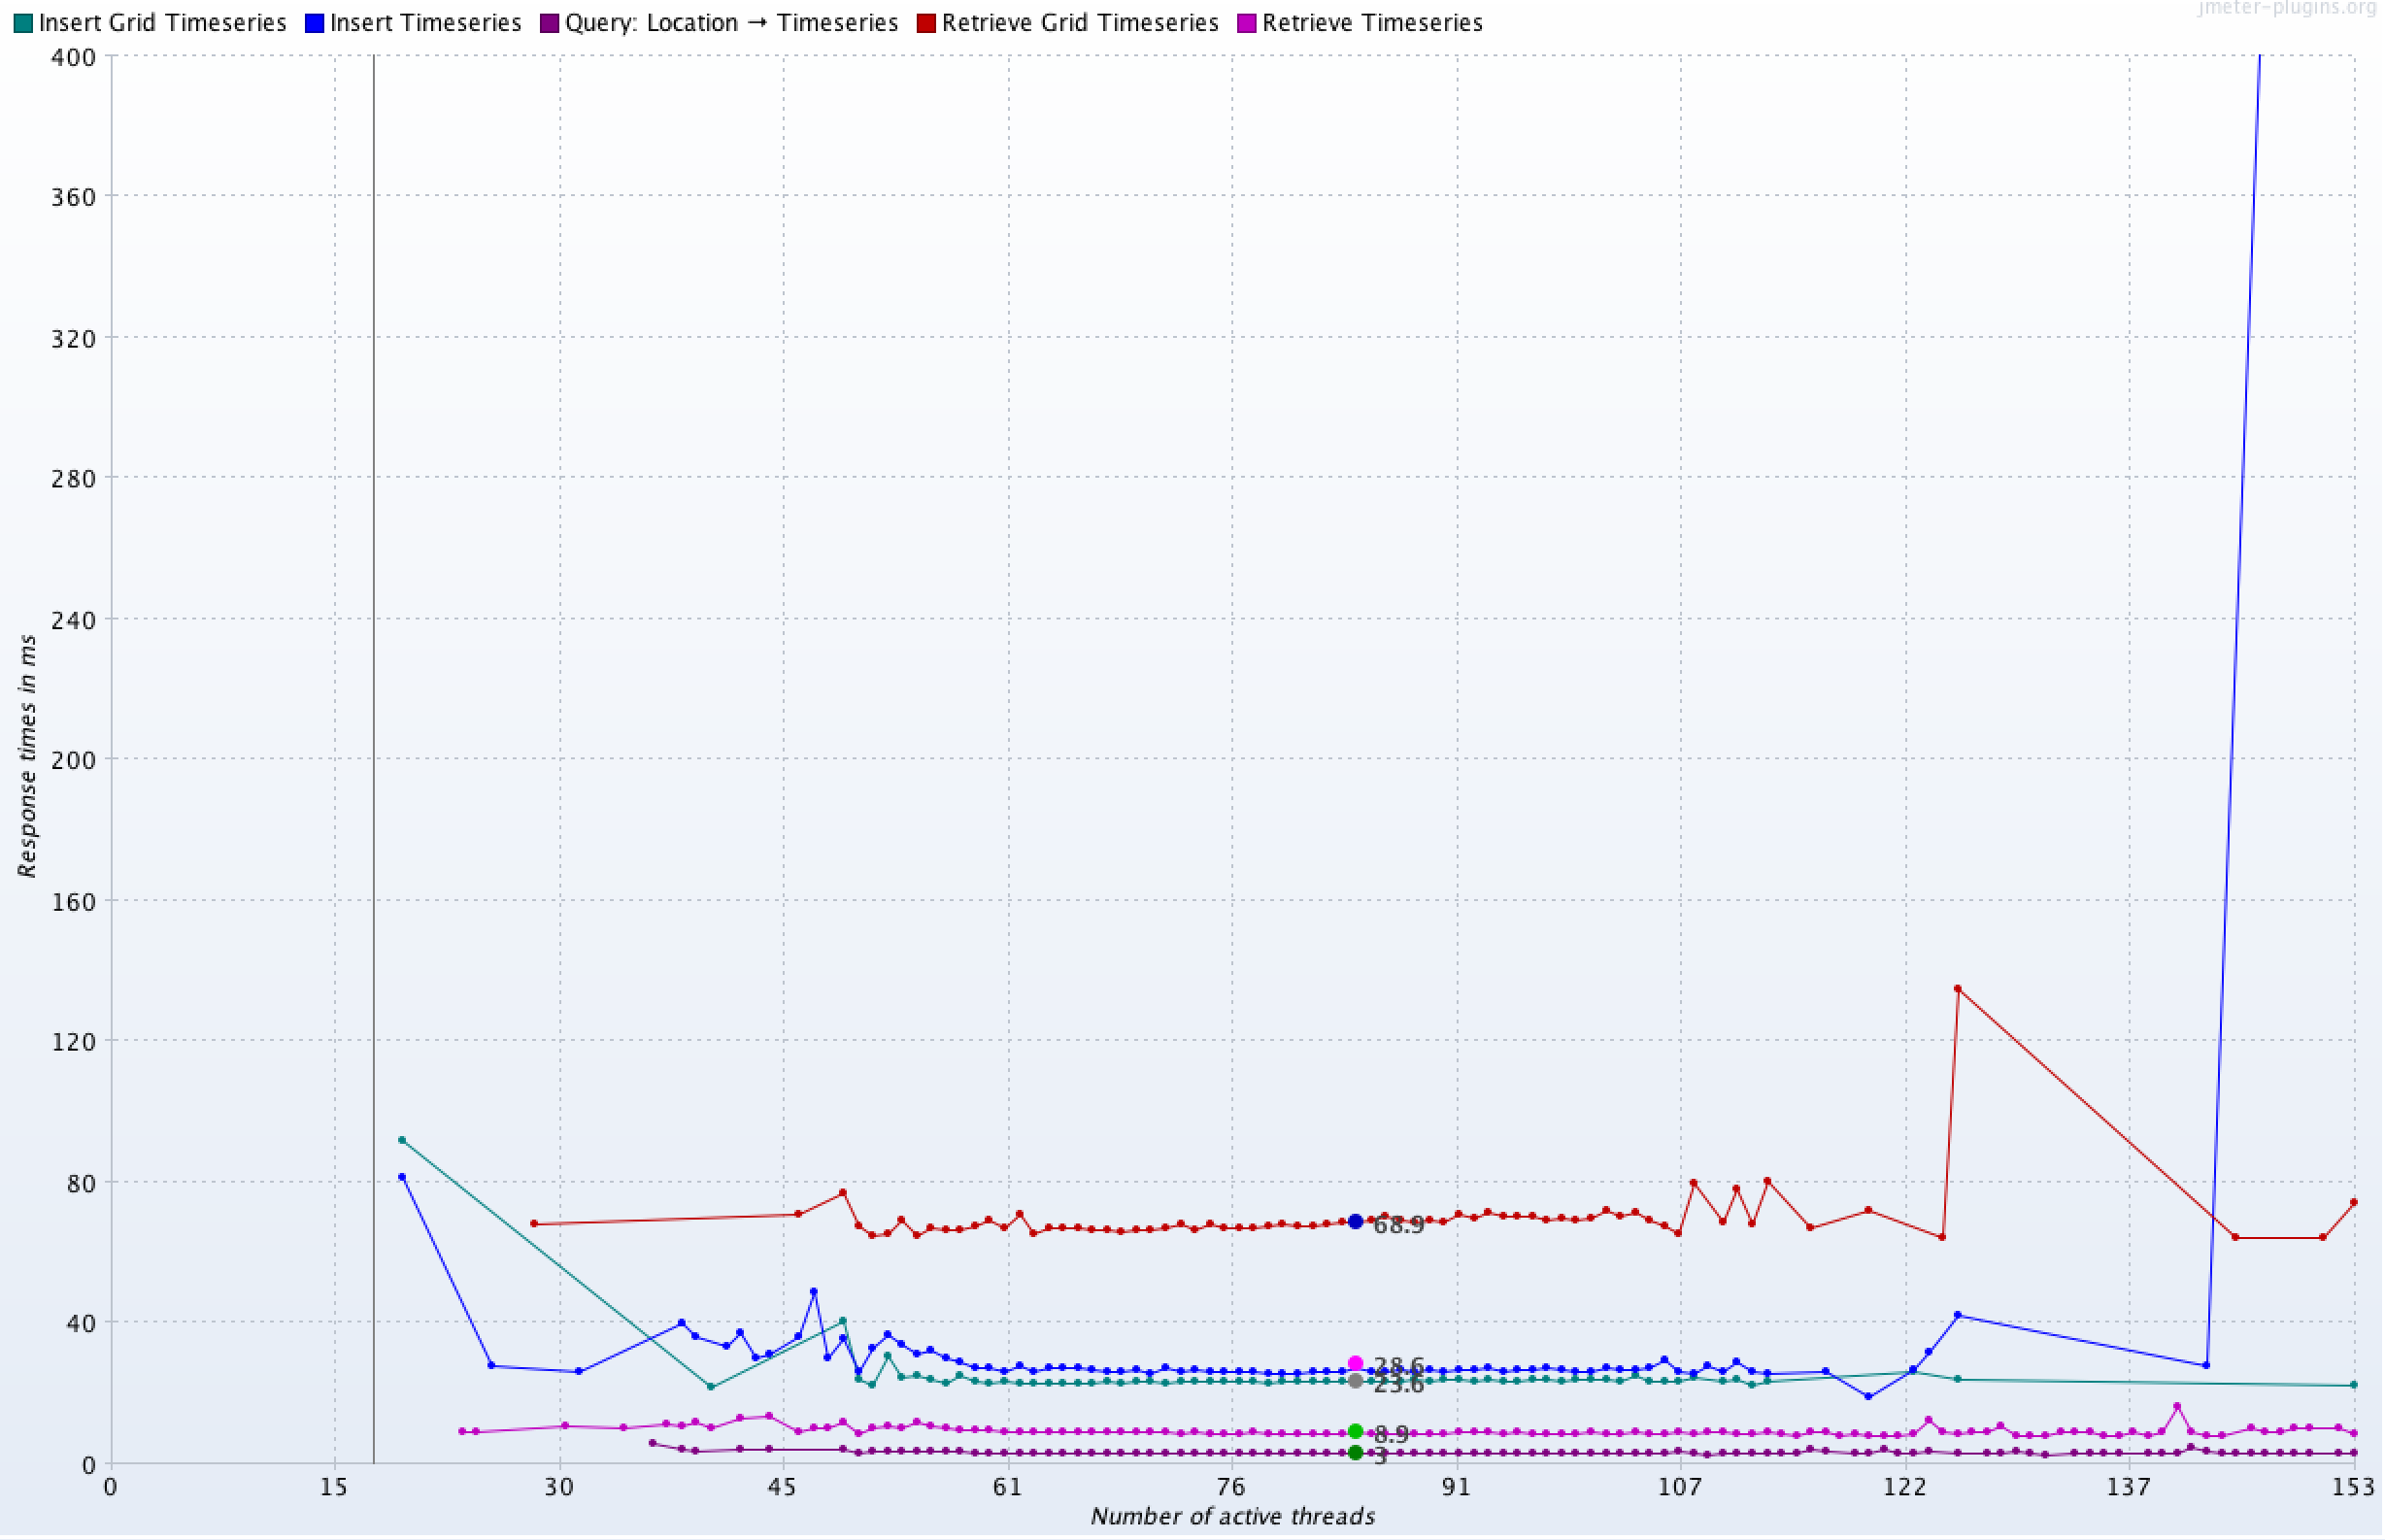
\includegraphics[width=0.8\textwidth]{results/obs/all/obs_all_60m_response_times_vs_threads.png}
    \caption{Load testing with hourly data - Response Time vs Threads}
    \label{fi:test_obs_all_60m_response_vs_threads}
\end{figure}
\ref{fi:test_obs_all_60m_response_vs_threads} show the response time against the number of active threads. As the graph show, the response time kept same while increasing the number of active threads against each test case. This shows the scalability of the \acrshort{wdias}, since the system able to process more requests without a significant change in the latency.
When number of active threads increased more than 122, the \ref{fi:test_obs_all_60m_response_vs_threads} show uncertainty in the inserting and retrieving Scalar and Vector data.

\begin{figure}[htp]
    \centering
    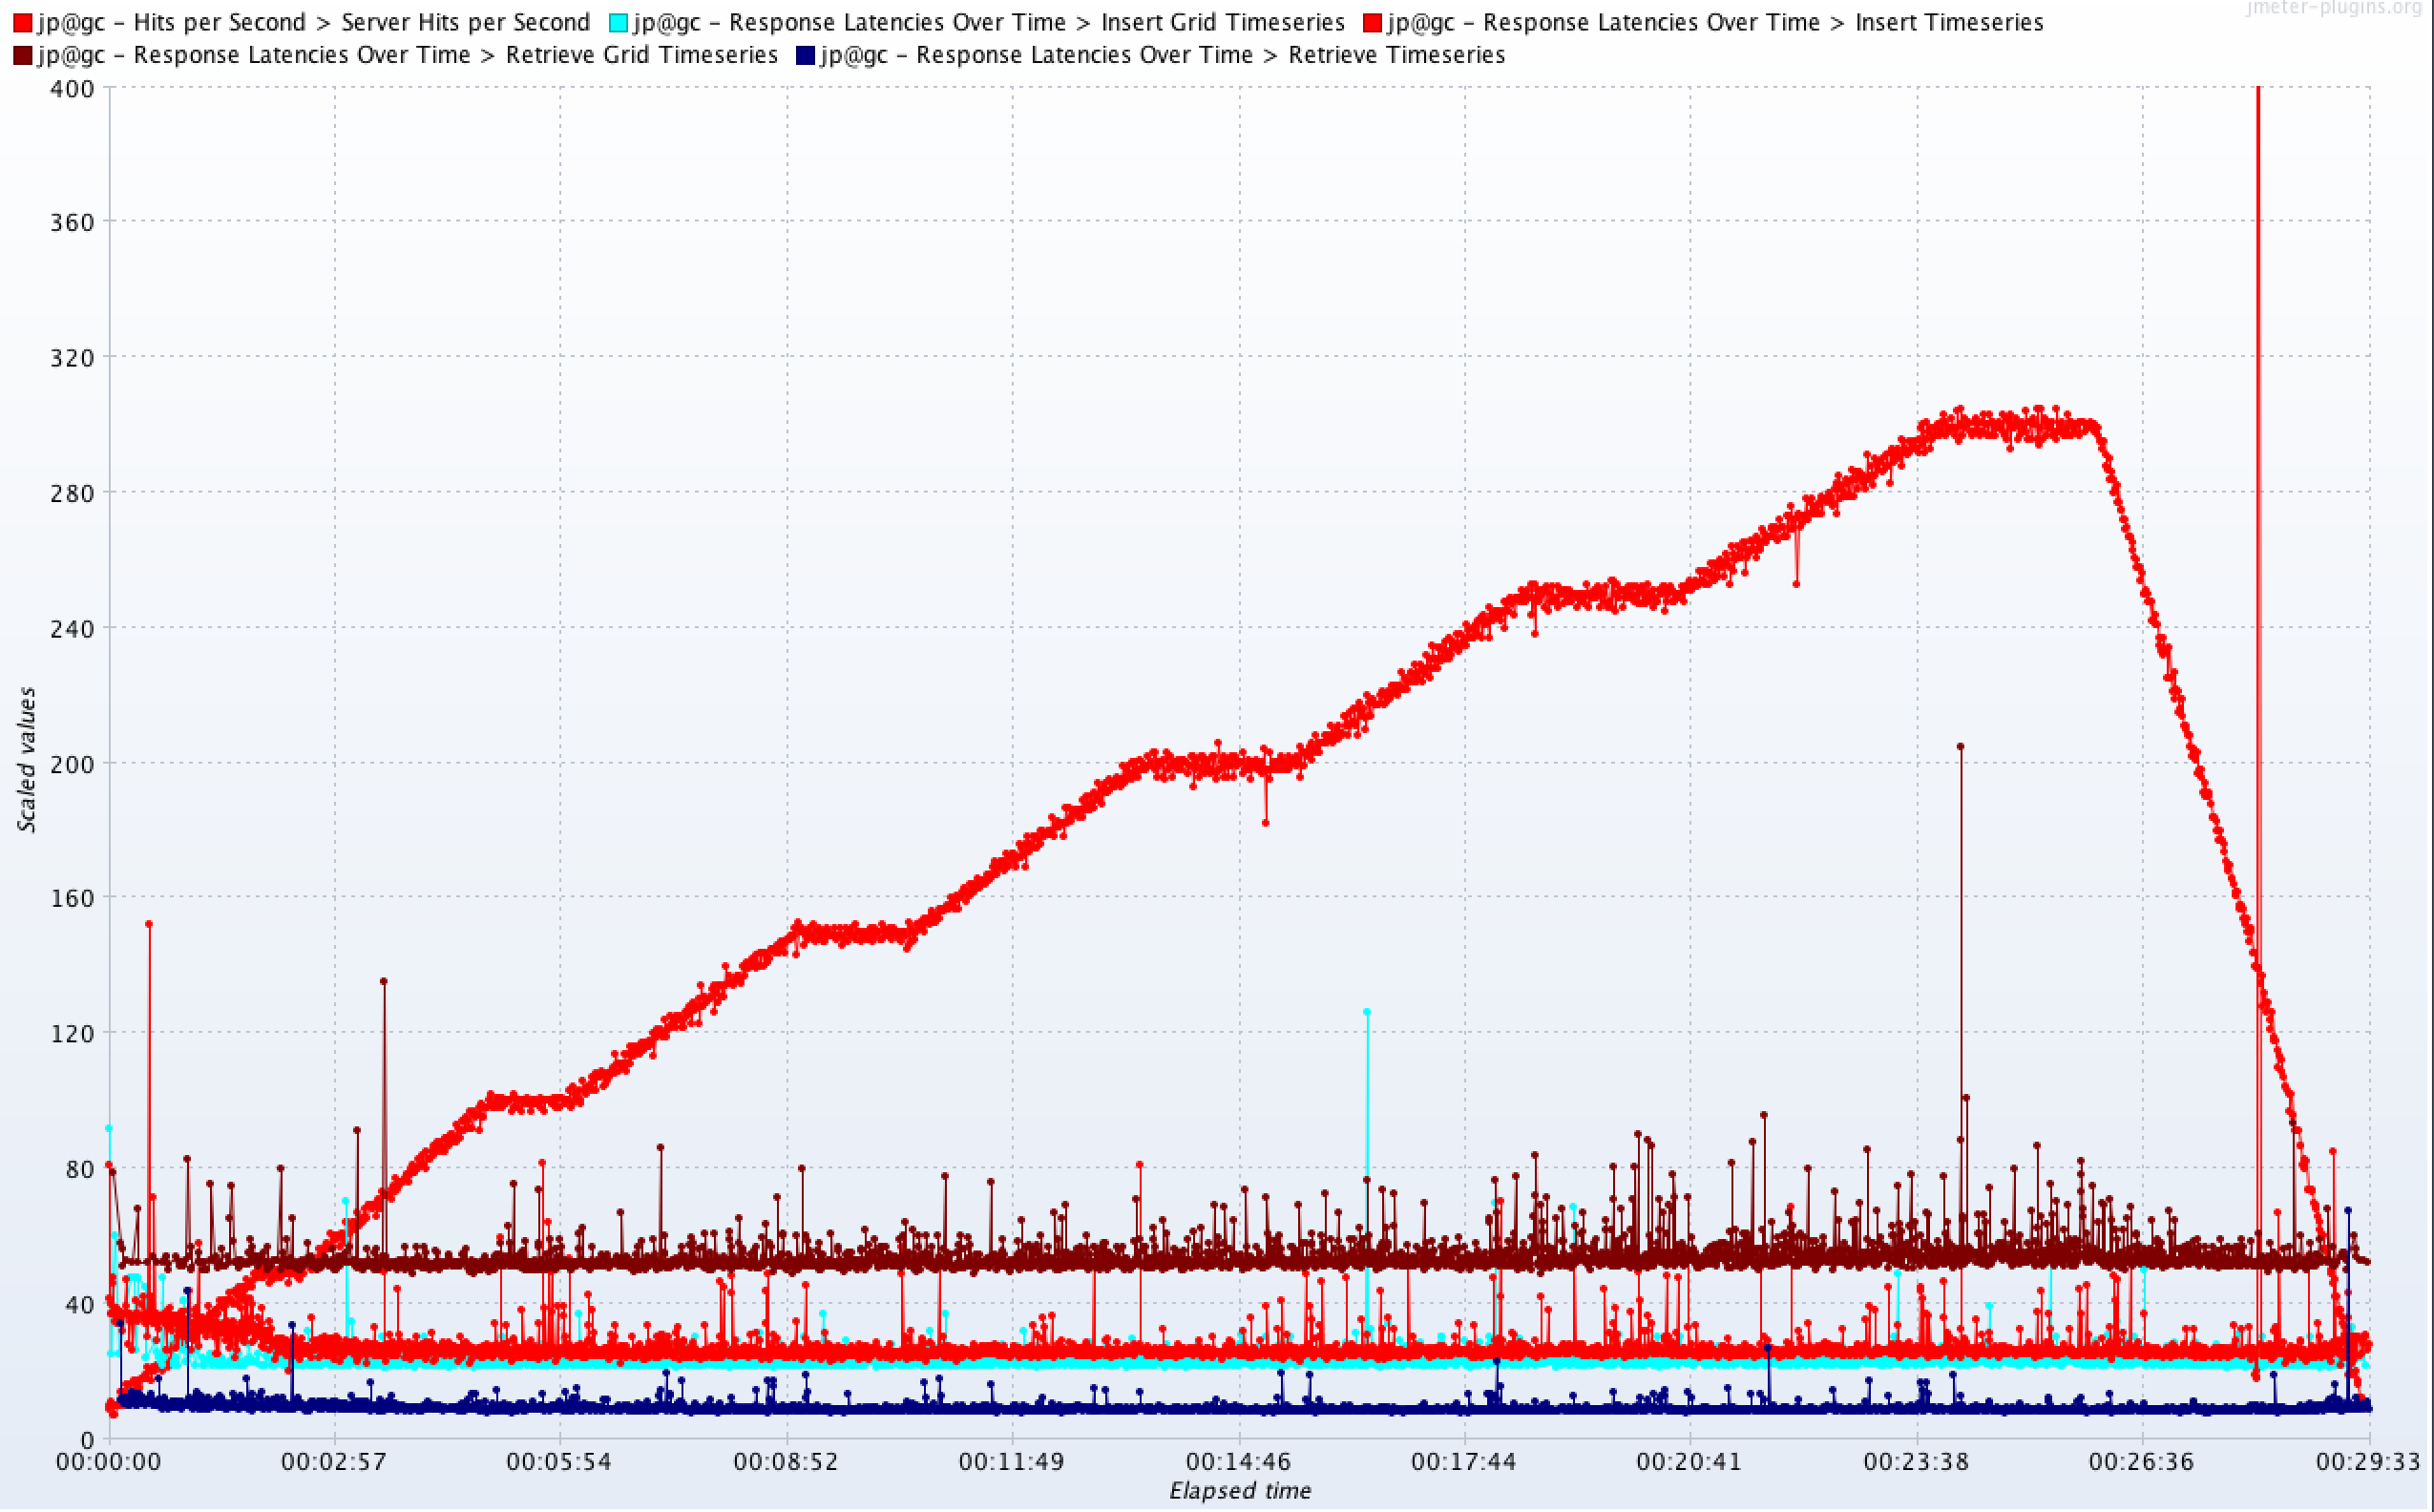
\includegraphics[width=0.8\textwidth]{results/obs/all/obs_all_60m_res_latencies_against_hits.png}
    \caption{Load testing with hourly data - Latency against server hits}
    \label{fi:test_obs_all_60m_latency}
\end{figure}
\ref{fi:test_obs_all_60m_latency} graph provides a better overview of the variation of latency over elapsed time of the test plan against number of server hits per second.
The conclusion of giving static latency while increasing the number of requests in \ref{fi:test_obs_all_60m_response_vs_threads} can further prove with this graph, since \ref{fi:test_obs_all_60m_latency} graph gives in details overview over the test plan time span.


%%%%%%%%%%%%%%%%%%%%%%%%%%%%%%%%%%%%%%%%%%%%%%%%%%%%%%%%%%%%%%%%%%%%%%%%%%%%%%%%
\subsection{Load Testing with 30min data (48 Request Size)}
\label{subse:obs_test_plan_all_30min}
This section \ref{subse:obs_test_plan_all_30min} discussed about the All test plan performance with 30 minutes data which means 48 data points per each request in Scalar and Vector timeseries, and 48 ASCII Grid files per each insert request. It performed round up to 311k of sample requests which is almost similar to \ref{subse:obs_test_plan_all_60min} processed samples.

\begin{table}[ht]
\caption{Throughput and Latency of load test with 30min data}
\footnotesize
\begin{tabulary}{\linewidth}{|L|C|C|C|C|C|C|C|C|}
\hline
Label & \# Samples & Average & Min & Max & 90\% Line & Std. Dev. & Error \% & RPS \\ \hline
Insert Timeseries & 71759 & 29 & 14 & 1699 & 32 & 50.97 & 0.00\% & 40.5 \\ \hline
Retrieve Timeseries & 71730 & 9 & 7 & 1033 & 10 & 6.04 & 0.00\% & 40.6 \\ \hline
Insert Grid & 7972 & 44 & 40 & 162 & 49 & 8.17 & 0.08\% & 4.5 \\ \hline
Retrieve Grid & 7971 & 81 & 67 & 284 & 93 & 15.15 & 0.00\% & 4.5 \\ \hline
Query: Location & 71734 & 3 & 2 & 110 & 3 & 1.90 & 0.00\% & 40.5 \\ \hline
TOTAL & 310878 & 129 & 0 & 1699 & 503 & 207.10 & 0.00\% & 175.3 \\ \hline
\end{tabulary}
\label{tab:obs_all_30_min_summary}
\end{table}
\ref{tab:obs_all_30_min_summary} shows the response latency summary details and \acrshort{rps} as explained in \ref{subse:obs_test_plan_all_60min}. And the results are almost similar to the observations in \ref{tab:obs_all_60_min_summary}. This implies that, even the request size is increased, the \acrshort{wdias} can perform better same as the with smaller size of data.

\begin{figure}[htp]
    \centering
    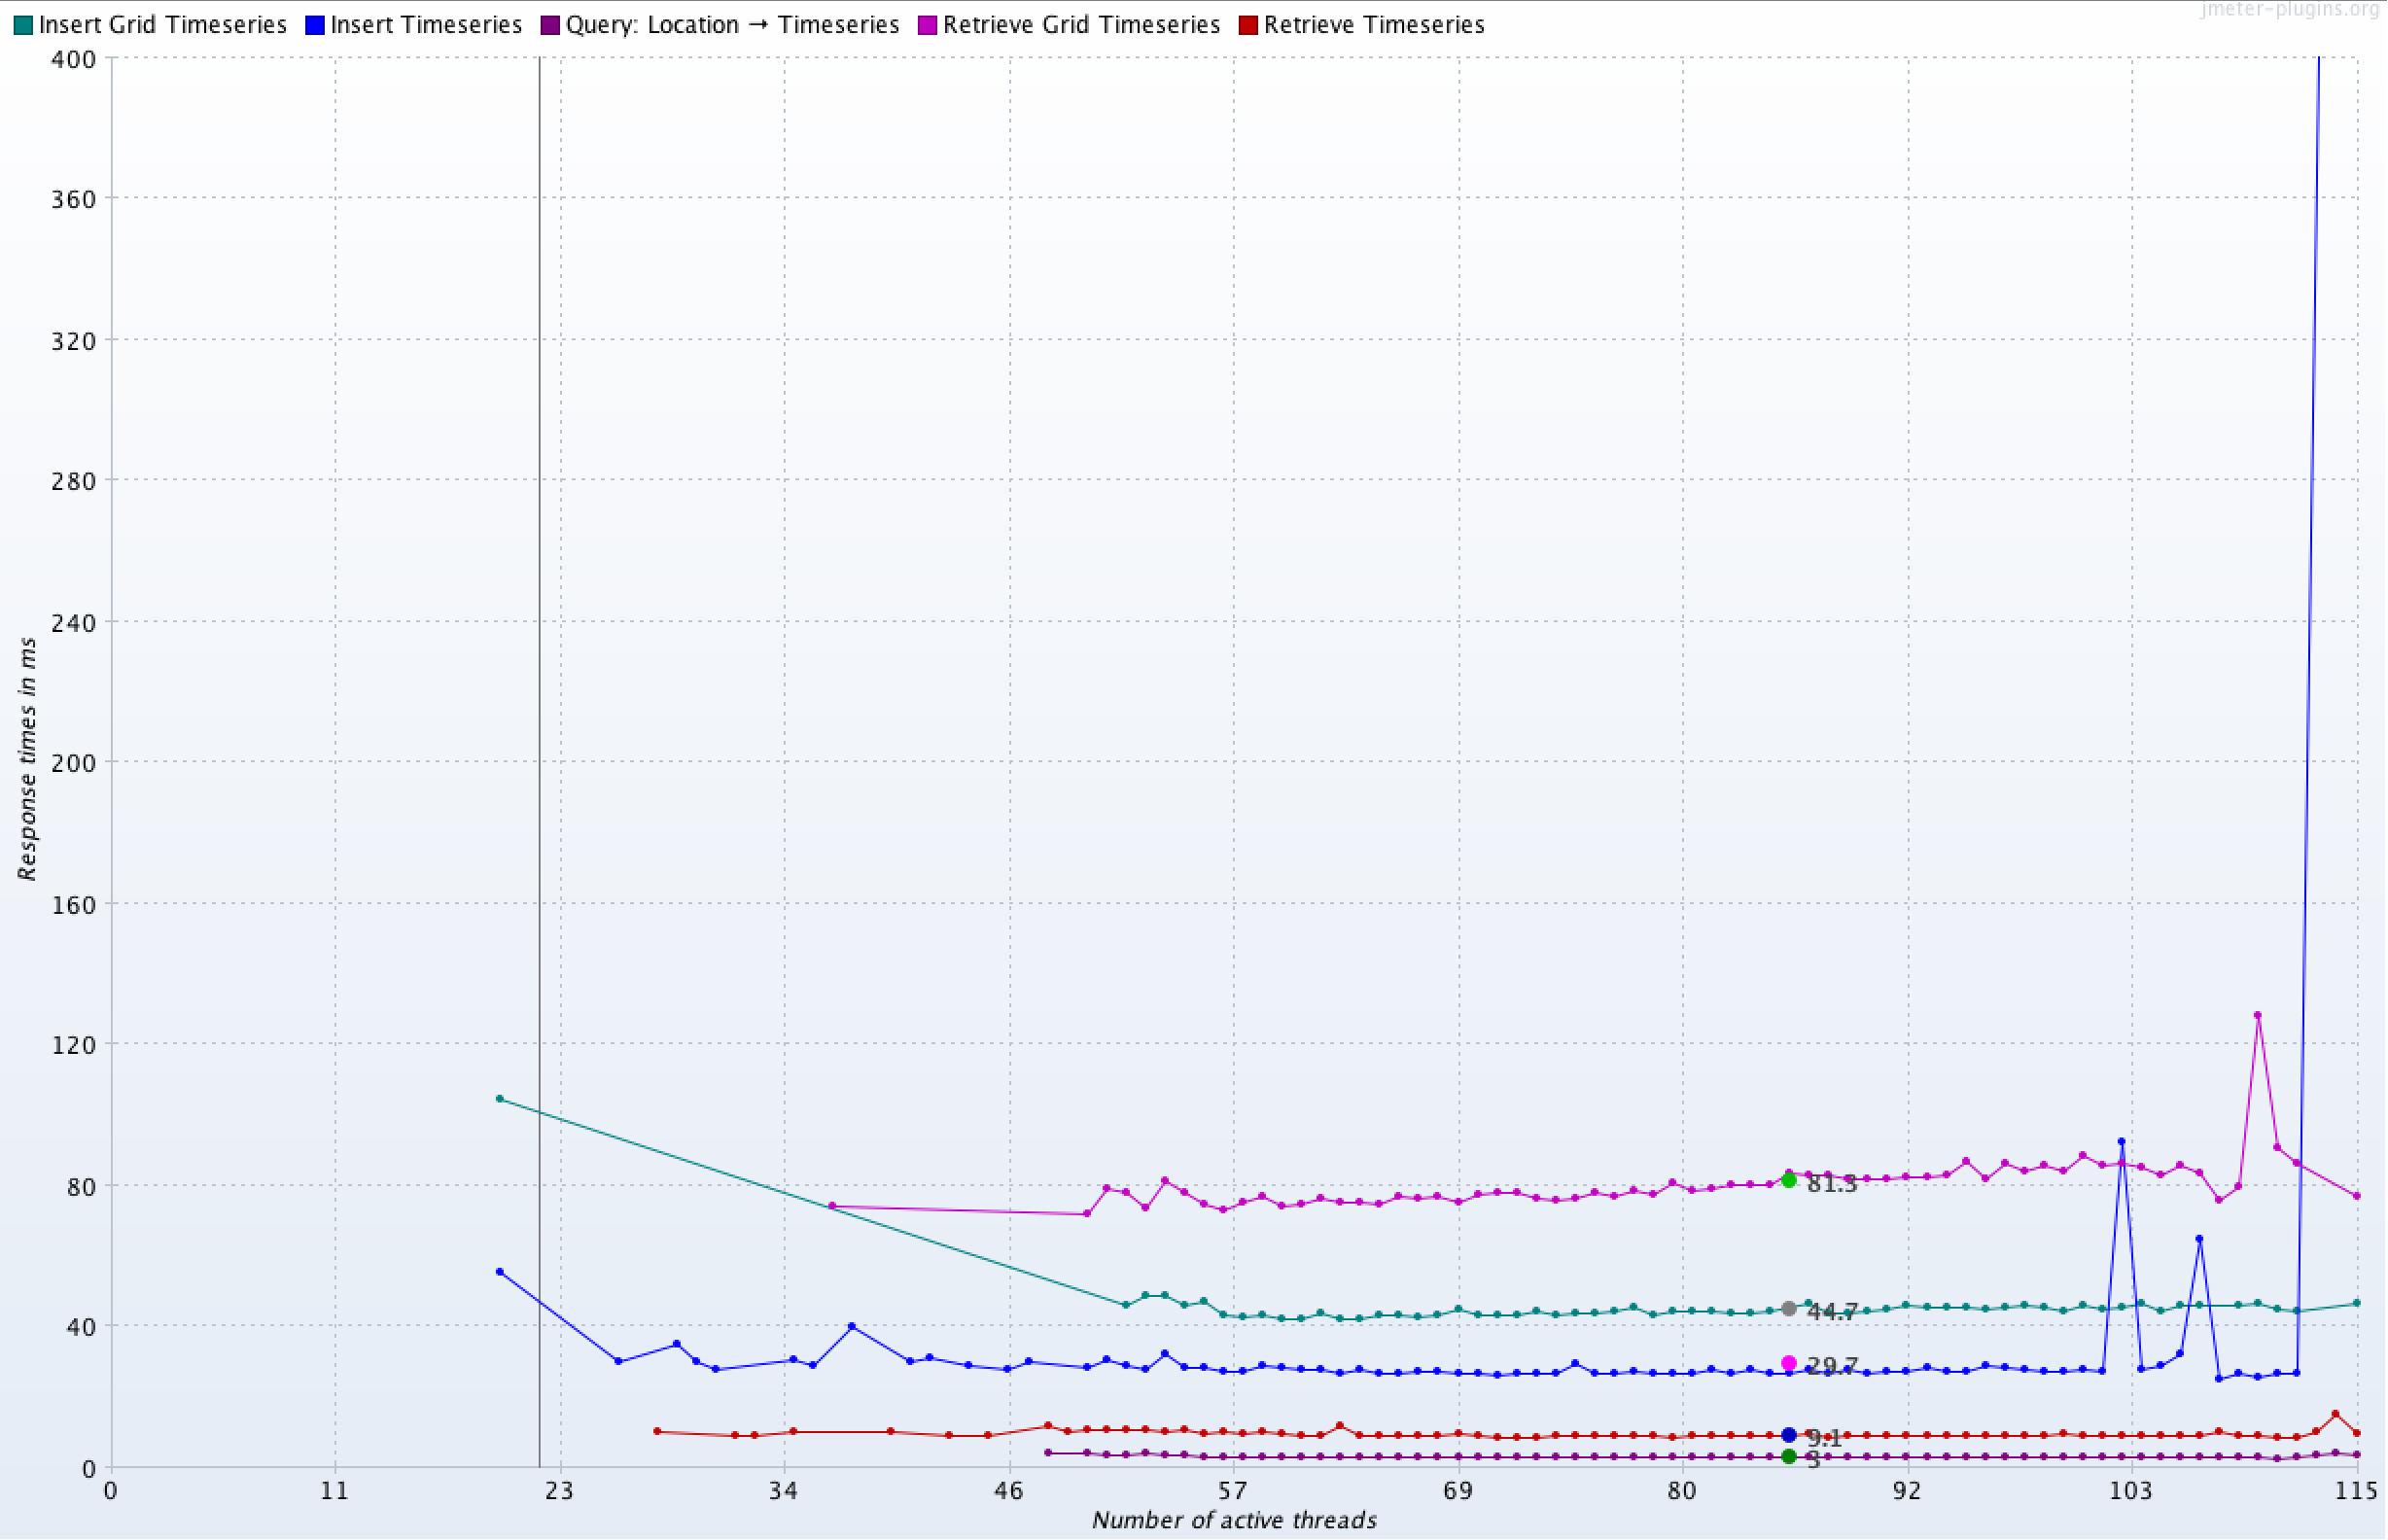
\includegraphics[width=0.8\textwidth]{results/obs/all/obs_all_30m_response_times_vs_threads.png}
    \caption{Load testing with 30 minutes data - Response Time vs Threads}
    \label{fi:test_obs_all_30m_response_vs_threads}
\end{figure}
\ref{fi:test_obs_all_30m_response_vs_threads} show the response time against the number of active threads for 30min data. As the graph show, the response time kept same while increasing the number of active threads against each test case. This shows the scalability of the \acrshort{wdias}, since the system able to process more requests without a significant change in the latency.
When number of active threads increased more than 110, the \ref{fi:test_obs_all_30m_response_vs_threads} show uncertainty in the inserting and retrieving Scalar and Vector data. This graph is similar to the \ref{fi:test_obs_all_60m_response_vs_threads}, but the active thread count goes down as a result of increasing the request size.

\begin{figure}[htp]
    \centering
    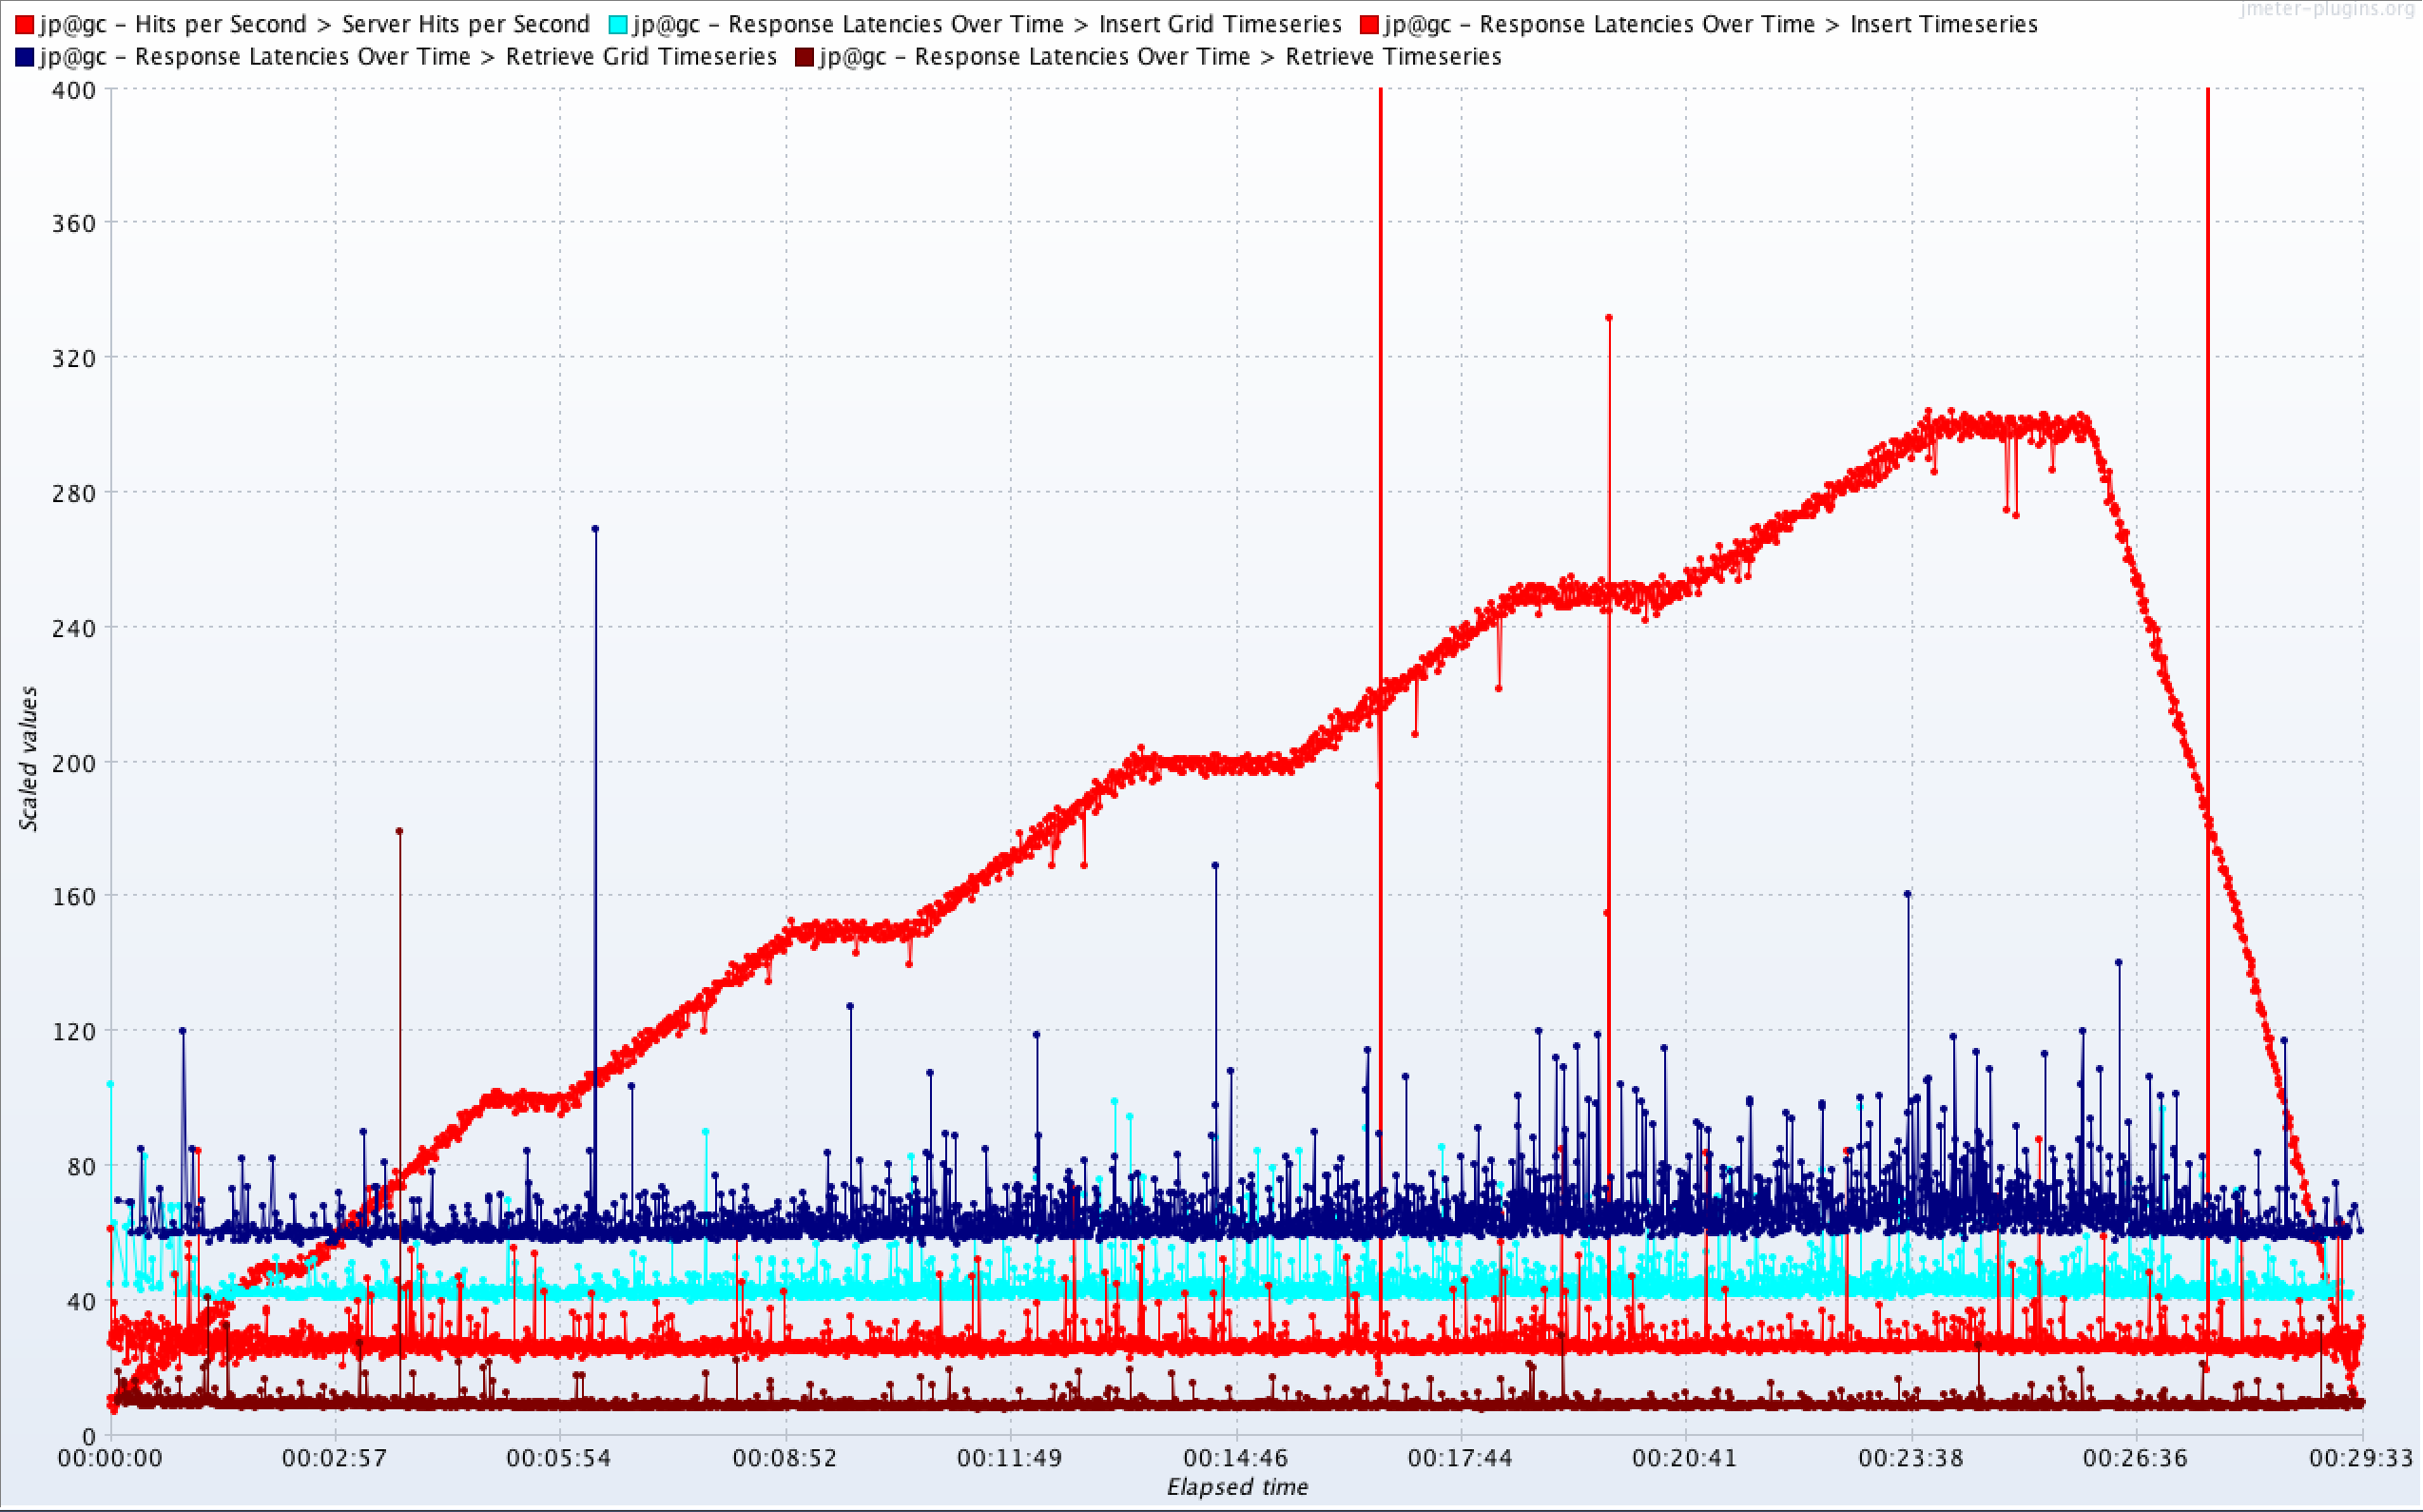
\includegraphics[width=0.8\textwidth]{results/obs/all/obs_all_30m_res_latencies_against_hits.png}
    \caption{Load testing with 30 minutes data - Latency against server hits}
    \label{fi:test_obs_all_30m_latency}
\end{figure}
\ref{fi:test_obs_all_30m_latency} graph provides a better overview of the variation of latency over elapsed time of the test plan against number of server hits per second.
This graph also conclude that, over the time latency does not change very much. But during the peak load, it shows some variation in insert and retrieve of Grid timeseries.
When compared to \ref{fi:test_obs_all_60m_latency}, the latency for insert and retrieve Grid timeseries increase by some amount.


%%%%%%%%%%%%%%%%%%%%%%%%%%%%%%%%%%%%%%%%%%%%%%%%%%%%%%%%%%%%%%%%%%%%%%%%%%%%%%%%
\subsection{Load Testing with 15min data (96 Request Size)}
\label{subse:obs_test_plan_all_15min}
This section \ref{subse:obs_test_plan_all_15min} discussed about the All test plan performance with 15 minutes data which means 96 data points per each request in Scalar and Vector timeseries, and 96 ASCII Grid files per each insert Grid timeseries request. These requests are four times larger than the \ref{subse:obs_test_plan_all_60min} request size. It performed approximately 311k of sample requests which is almost similar to \ref{subse:obs_test_plan_all_30min} processed samples.
\begin{table}[ht]
\caption{Throughput and Latency of load testing with 15min data}
\footnotesize
\begin{tabulary}{\linewidth}{|L|C|C|C|C|C|C|C|C|}
\hline
Label & \# Samples & Average & Min & Max & 90\% Line & Std. Dev. & Error \% & RPS \\ \hline
Insert Timeseries & 71775 & 30 & 12 & 1719 & 41 & 51.71 & 0.00\% & 40.5 \\ \hline
Retrieve Timeseries & 71736 & 23 & 8 & 1623 & 32 & 50.18 & 0.00\% & 40.6 \\ \hline
Insert Grid & 7975 & 91 & 77 & 279 & 112 & 19.58 & 1.42\% & 4.5 \\ \hline
Retrieve Grid & 7972 & 118 & 80 & 876 & 165 & 56.15 & 0.00\% & 4.5 \\ \hline
Query: Location & 71749 & 3 & 2 & 130 & 4 & 2.32 & 0.00\% & 40.5 \\ \hline
\textbf{TOTAL} & 310934 & 134 & 0 & 1719 & 503 & 206.40 & 0.04\% & 175.4 \\ \hline
\end{tabulary}
\label{tab:obs_all_15_min_summary}
\end{table}
\ref{tab:obs_all_15_min_summary} shows the response latency summary details and \acrshort{rps} as same as explained in \ref{subse:obs_test_plan_all_30min}. And the latency observations are increased by some amount when compared to the observations in \ref{tab:obs_all_30_min_summary}. Noticeably retrieving latency of all type of data types increased by considerable amount. Same following the trend, standard deviation of retrieve timeseries data increased my considerable amount for all the types. We can assume that more writing to the databases affected on reads as well. Event the request data size increased by 4x time, the \acrshort{wdias} were able to handle them without any significant performance issues. And the system able to provide the same throughput as \ref{tab:obs_all_30_min_summary}.

\begin{figure}[htp]
    \centering
    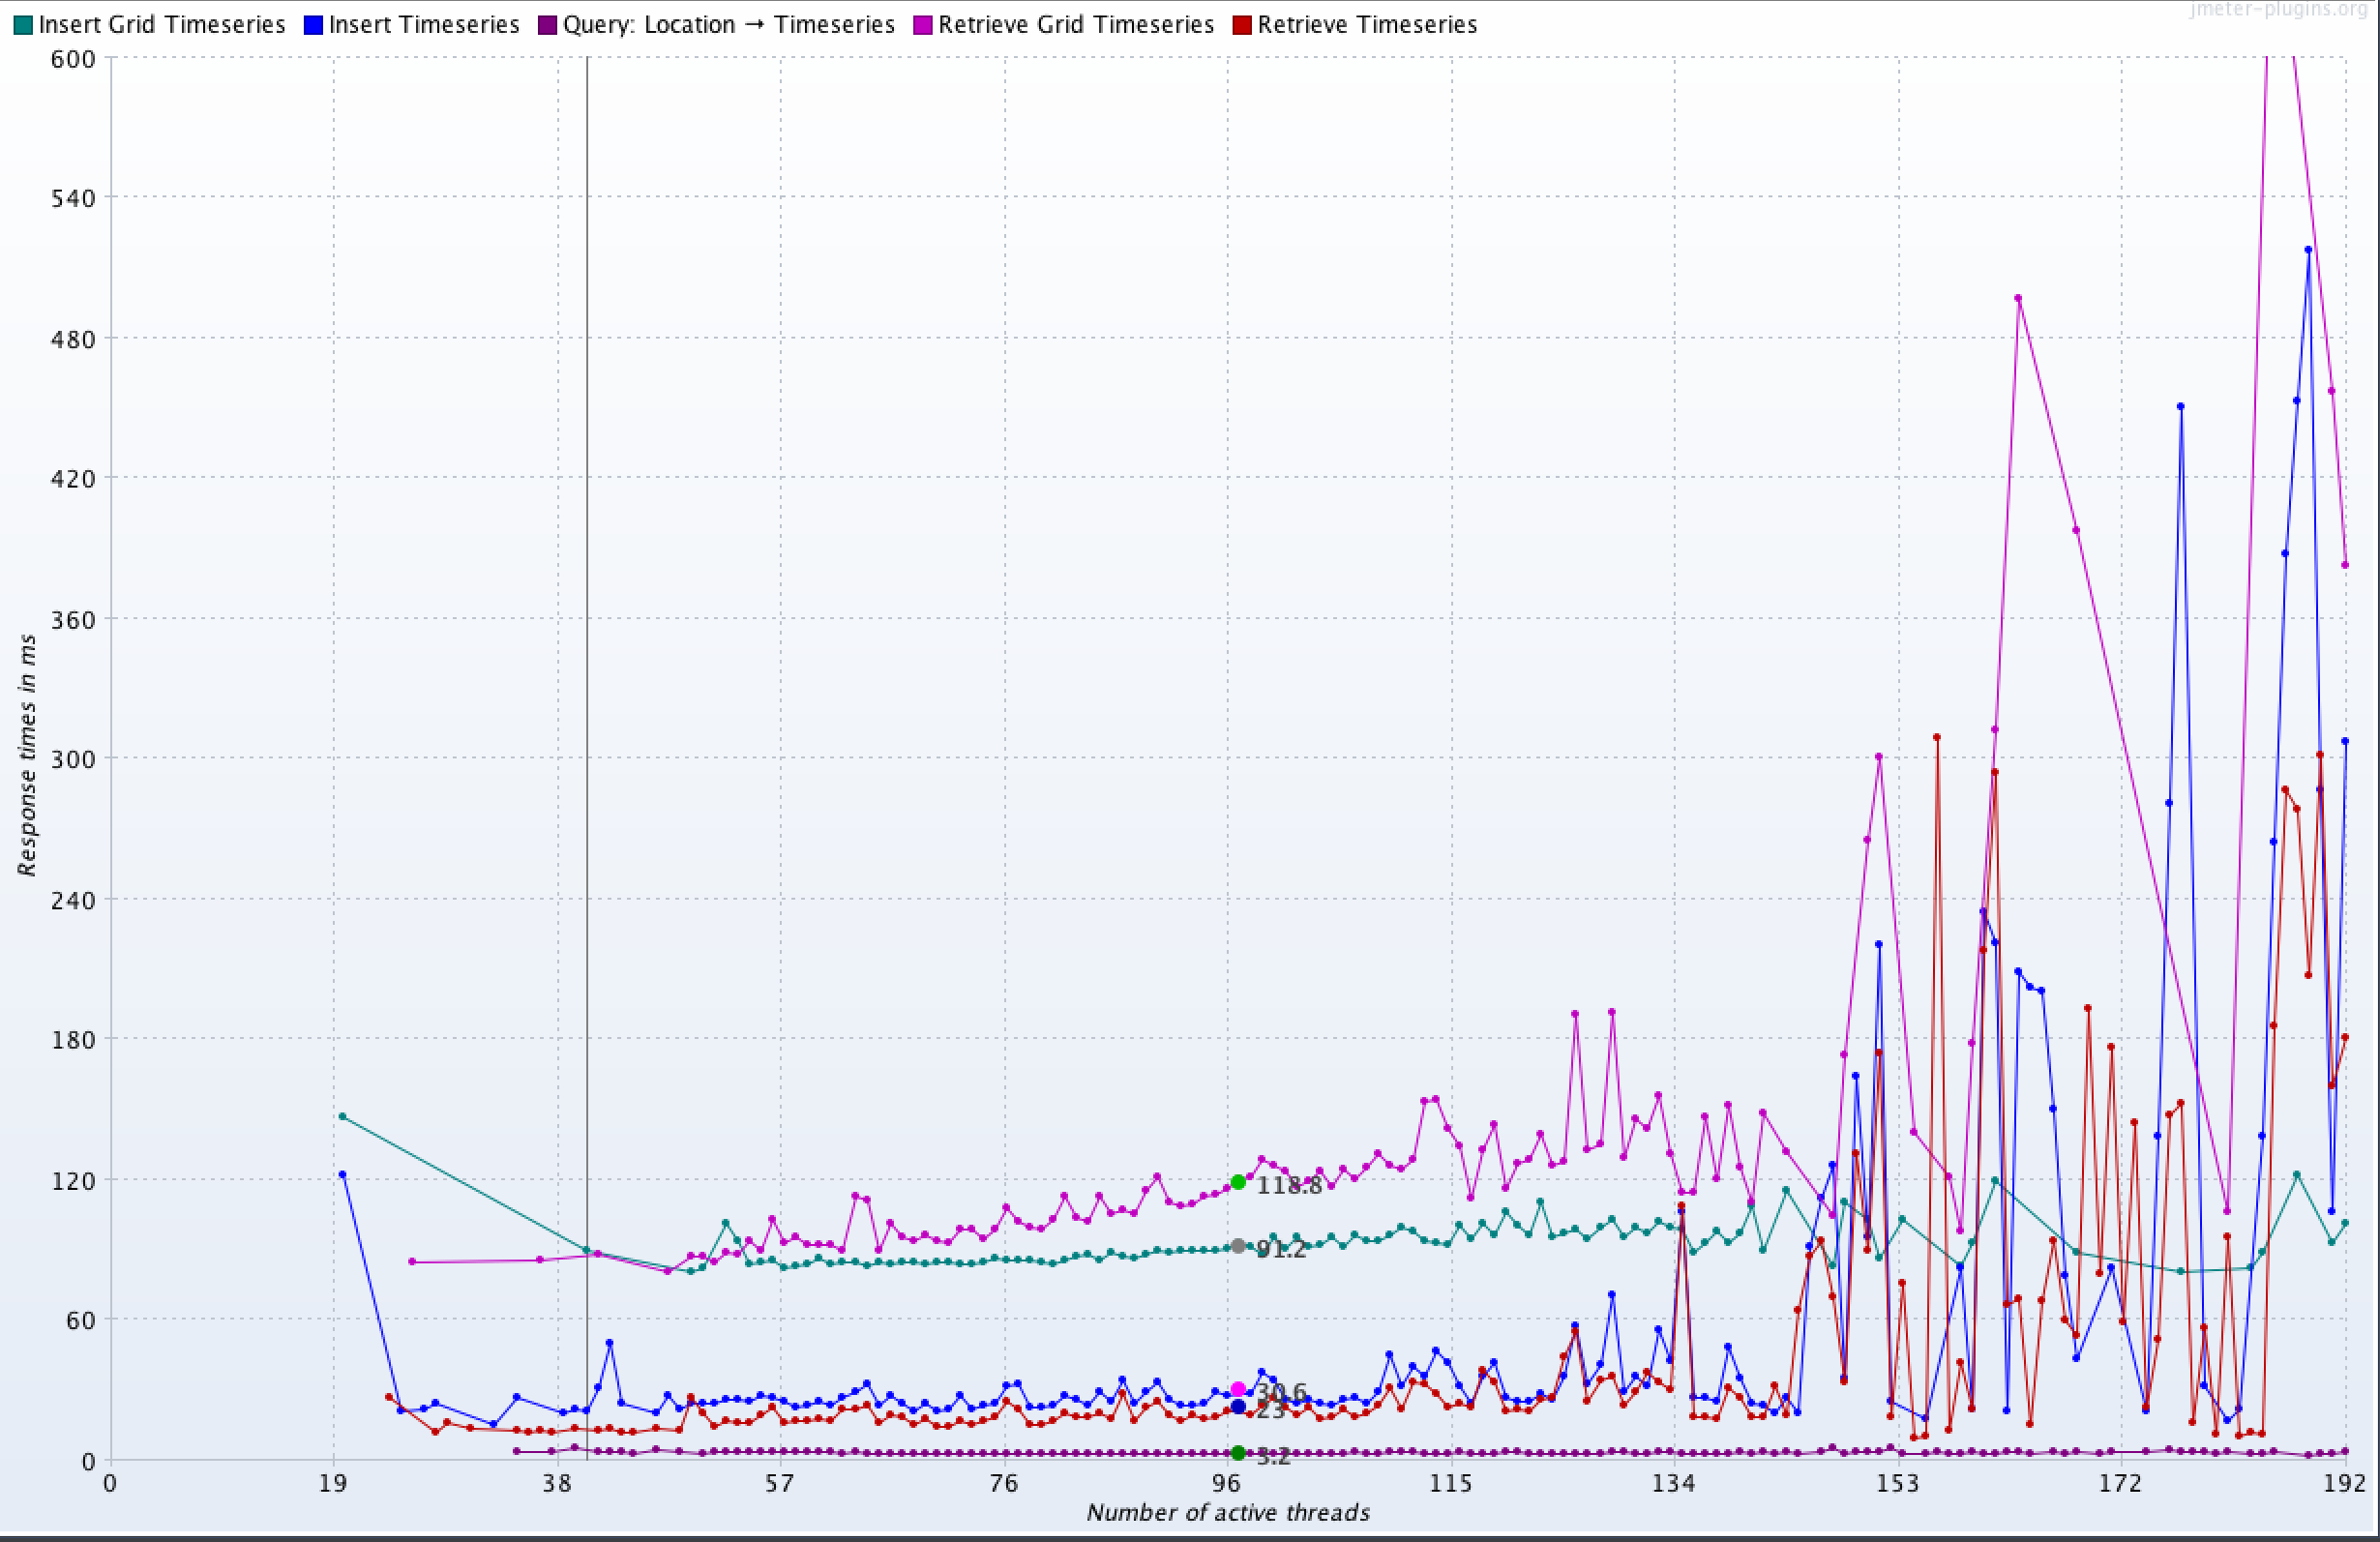
\includegraphics[width=0.8\textwidth]{results/obs/all/obs_all_15m_response_times_vs_threads.png}
    \caption{Load testing with 15 minutes data - Response Time vs Active Threads}
    \label{fi:test_obs_all_15m_response_vs_threads}
\end{figure}
\ref{fi:test_obs_all_15m_response_vs_threads} show the response time against the number of active threads for 15min data. As the graph show, the response time kept same while increasing the number of active threads against each test case. When number of active threads increased more than 140, the \ref{fi:test_obs_all_15m_response_vs_threads} show uncertainty in the inserting and retrieving all data types. The latency of insert and retrieve Grid timeseries data goes up compared to \ref{fi:test_obs_all_30m_response_vs_threads}.
With higher request size, it become to notice the latency also increase by a small factor when the number of active thread increased. This can clearly notice on with insert and retrieval of Grid timeseries data.

\begin{figure}[htp]
    \centering
    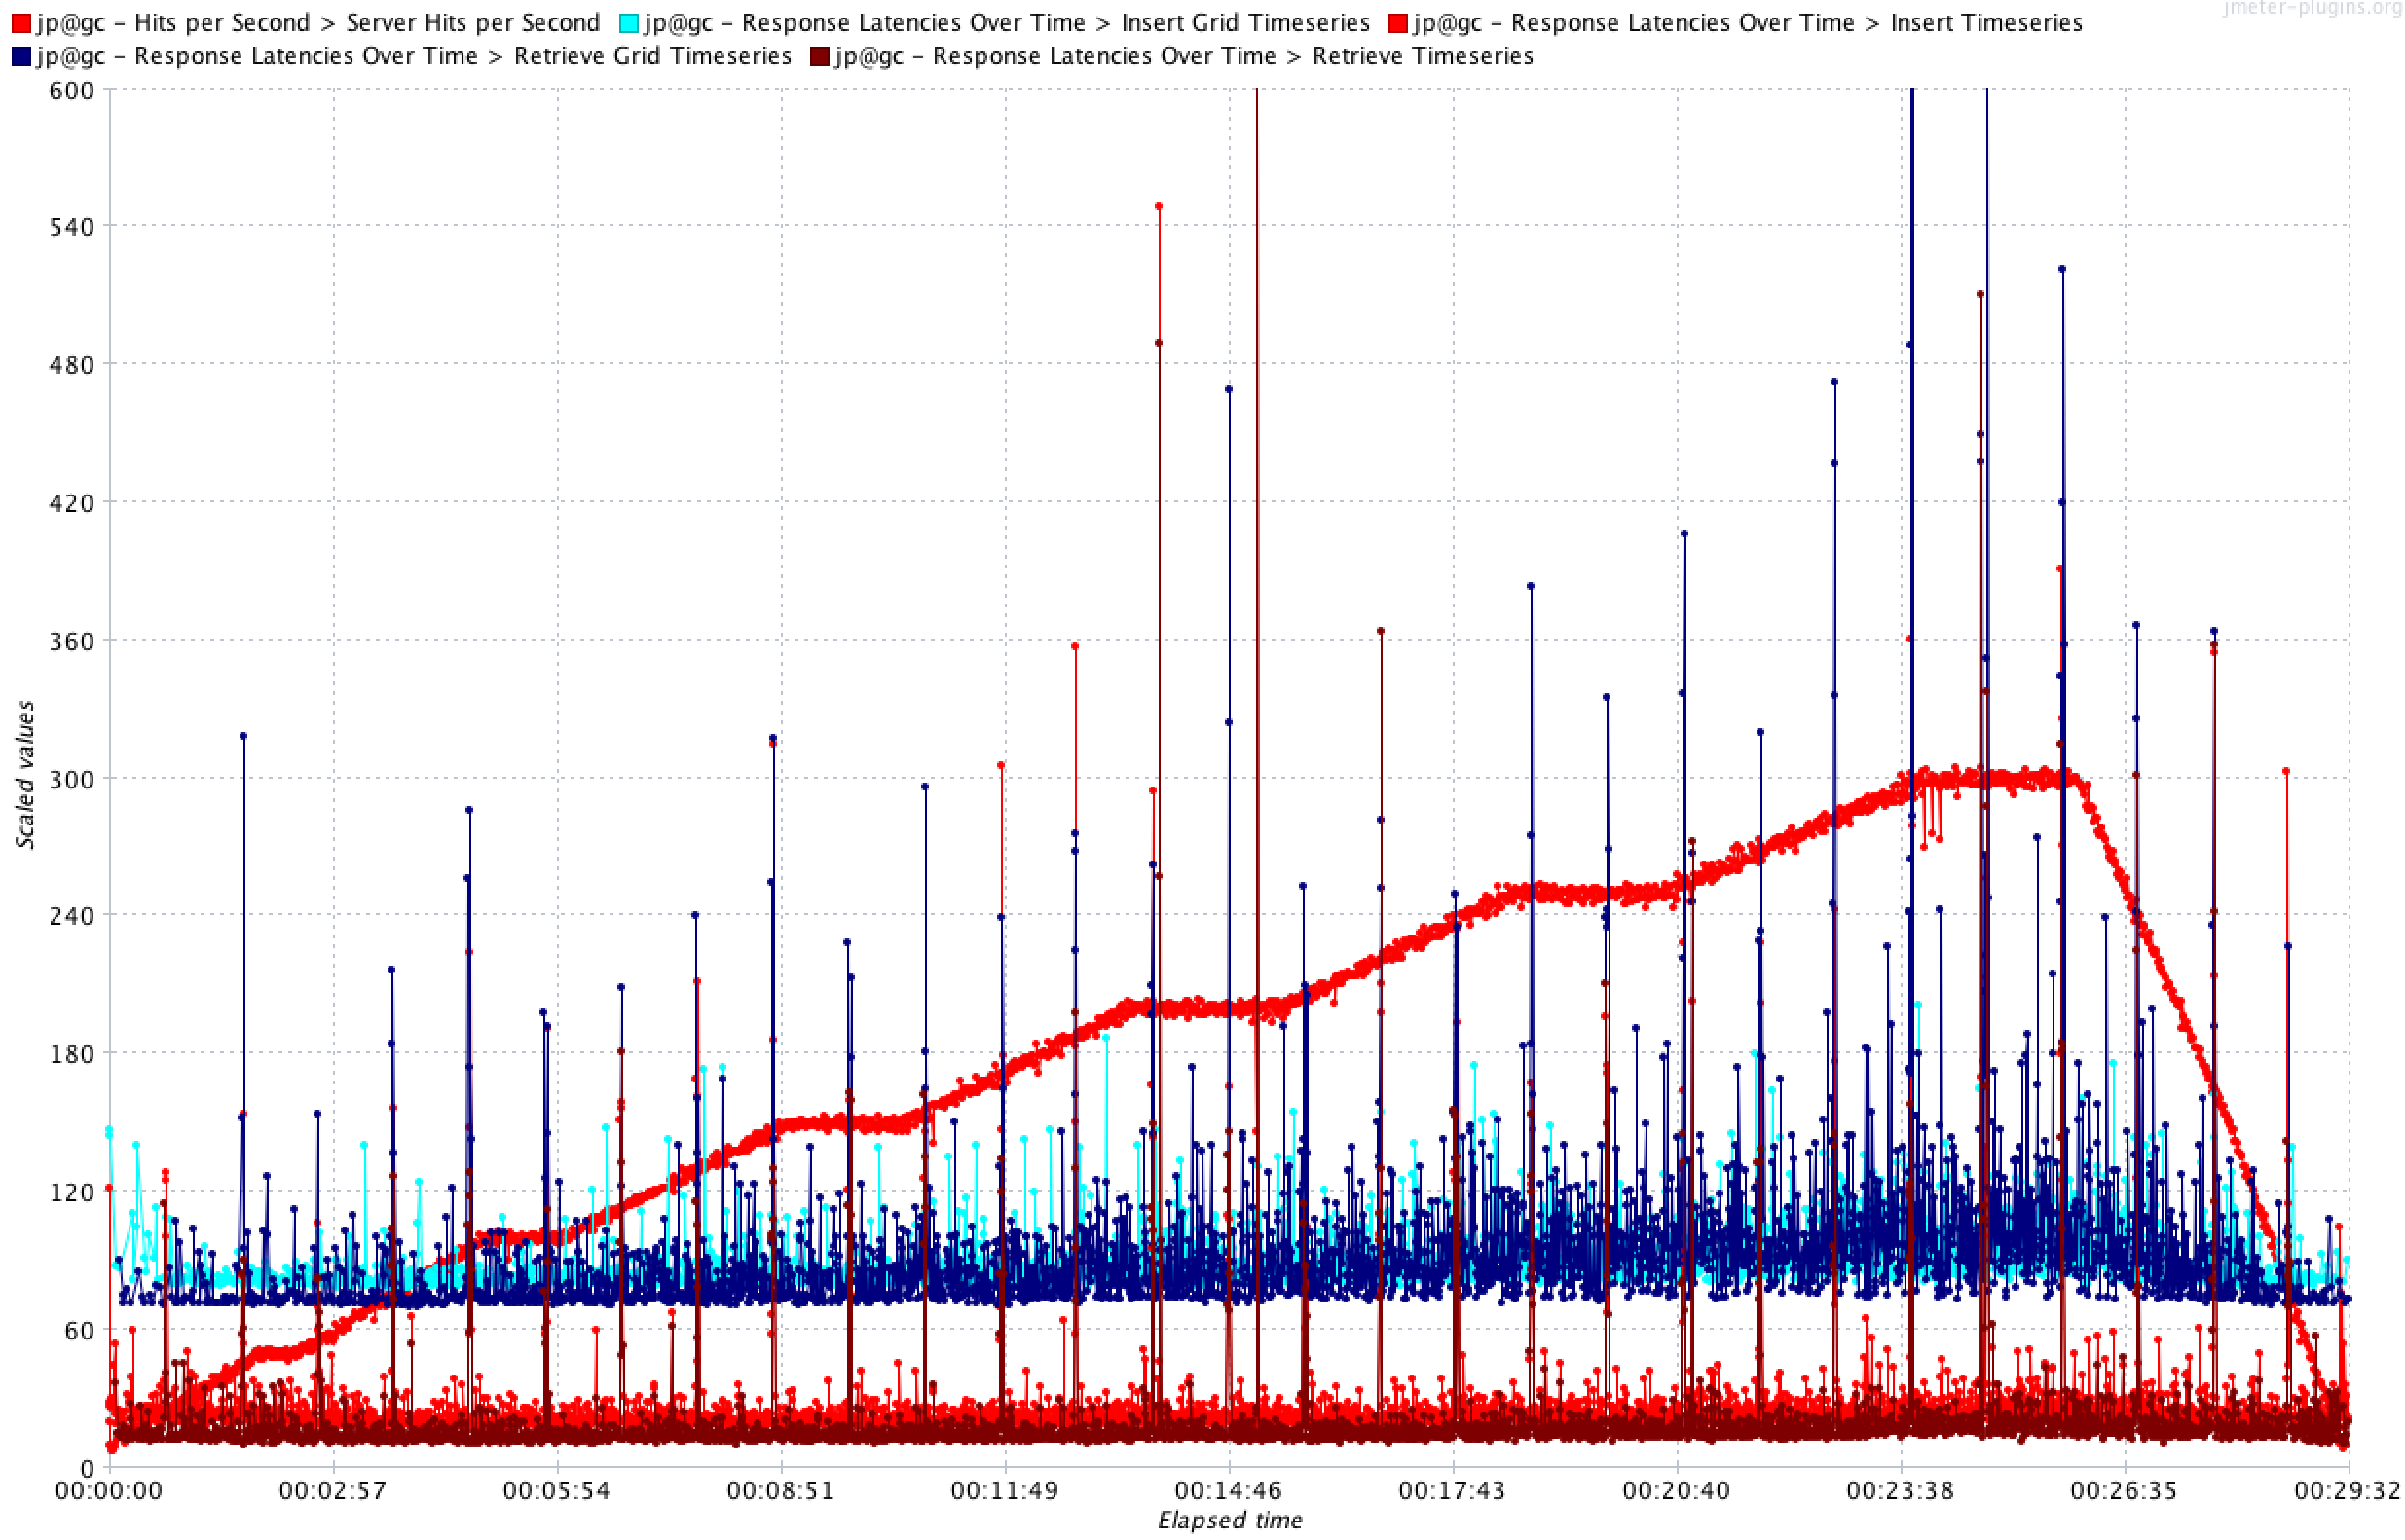
\includegraphics[width=0.8\textwidth]{results/obs/all/obs_all_15m_res_latencies_against_hits.png}
    \caption{Load testing with 15 minutes data - Latency against server hits}
    \label{fi:test_obs_all_15m_latency}
\end{figure}
\ref{fi:test_obs_all_15m_latency} graph provides a overview of the variation of latency over elapsed time of the test plan against number of server hits per second for 15min data.
This graph show that over the time \acrshort{wdias} were able to keep the latency constant over the test plan. But at the peak time, it tend to vary from the mean value a lot.
One noticeable fact is, throw out the test time period, it shows spikes in latency when compared to \ref{fi:test_obs_all_60m_latency} and \ref{fi:test_obs_all_30m_latency}.

\begin{figure}[htp]
    \centering
    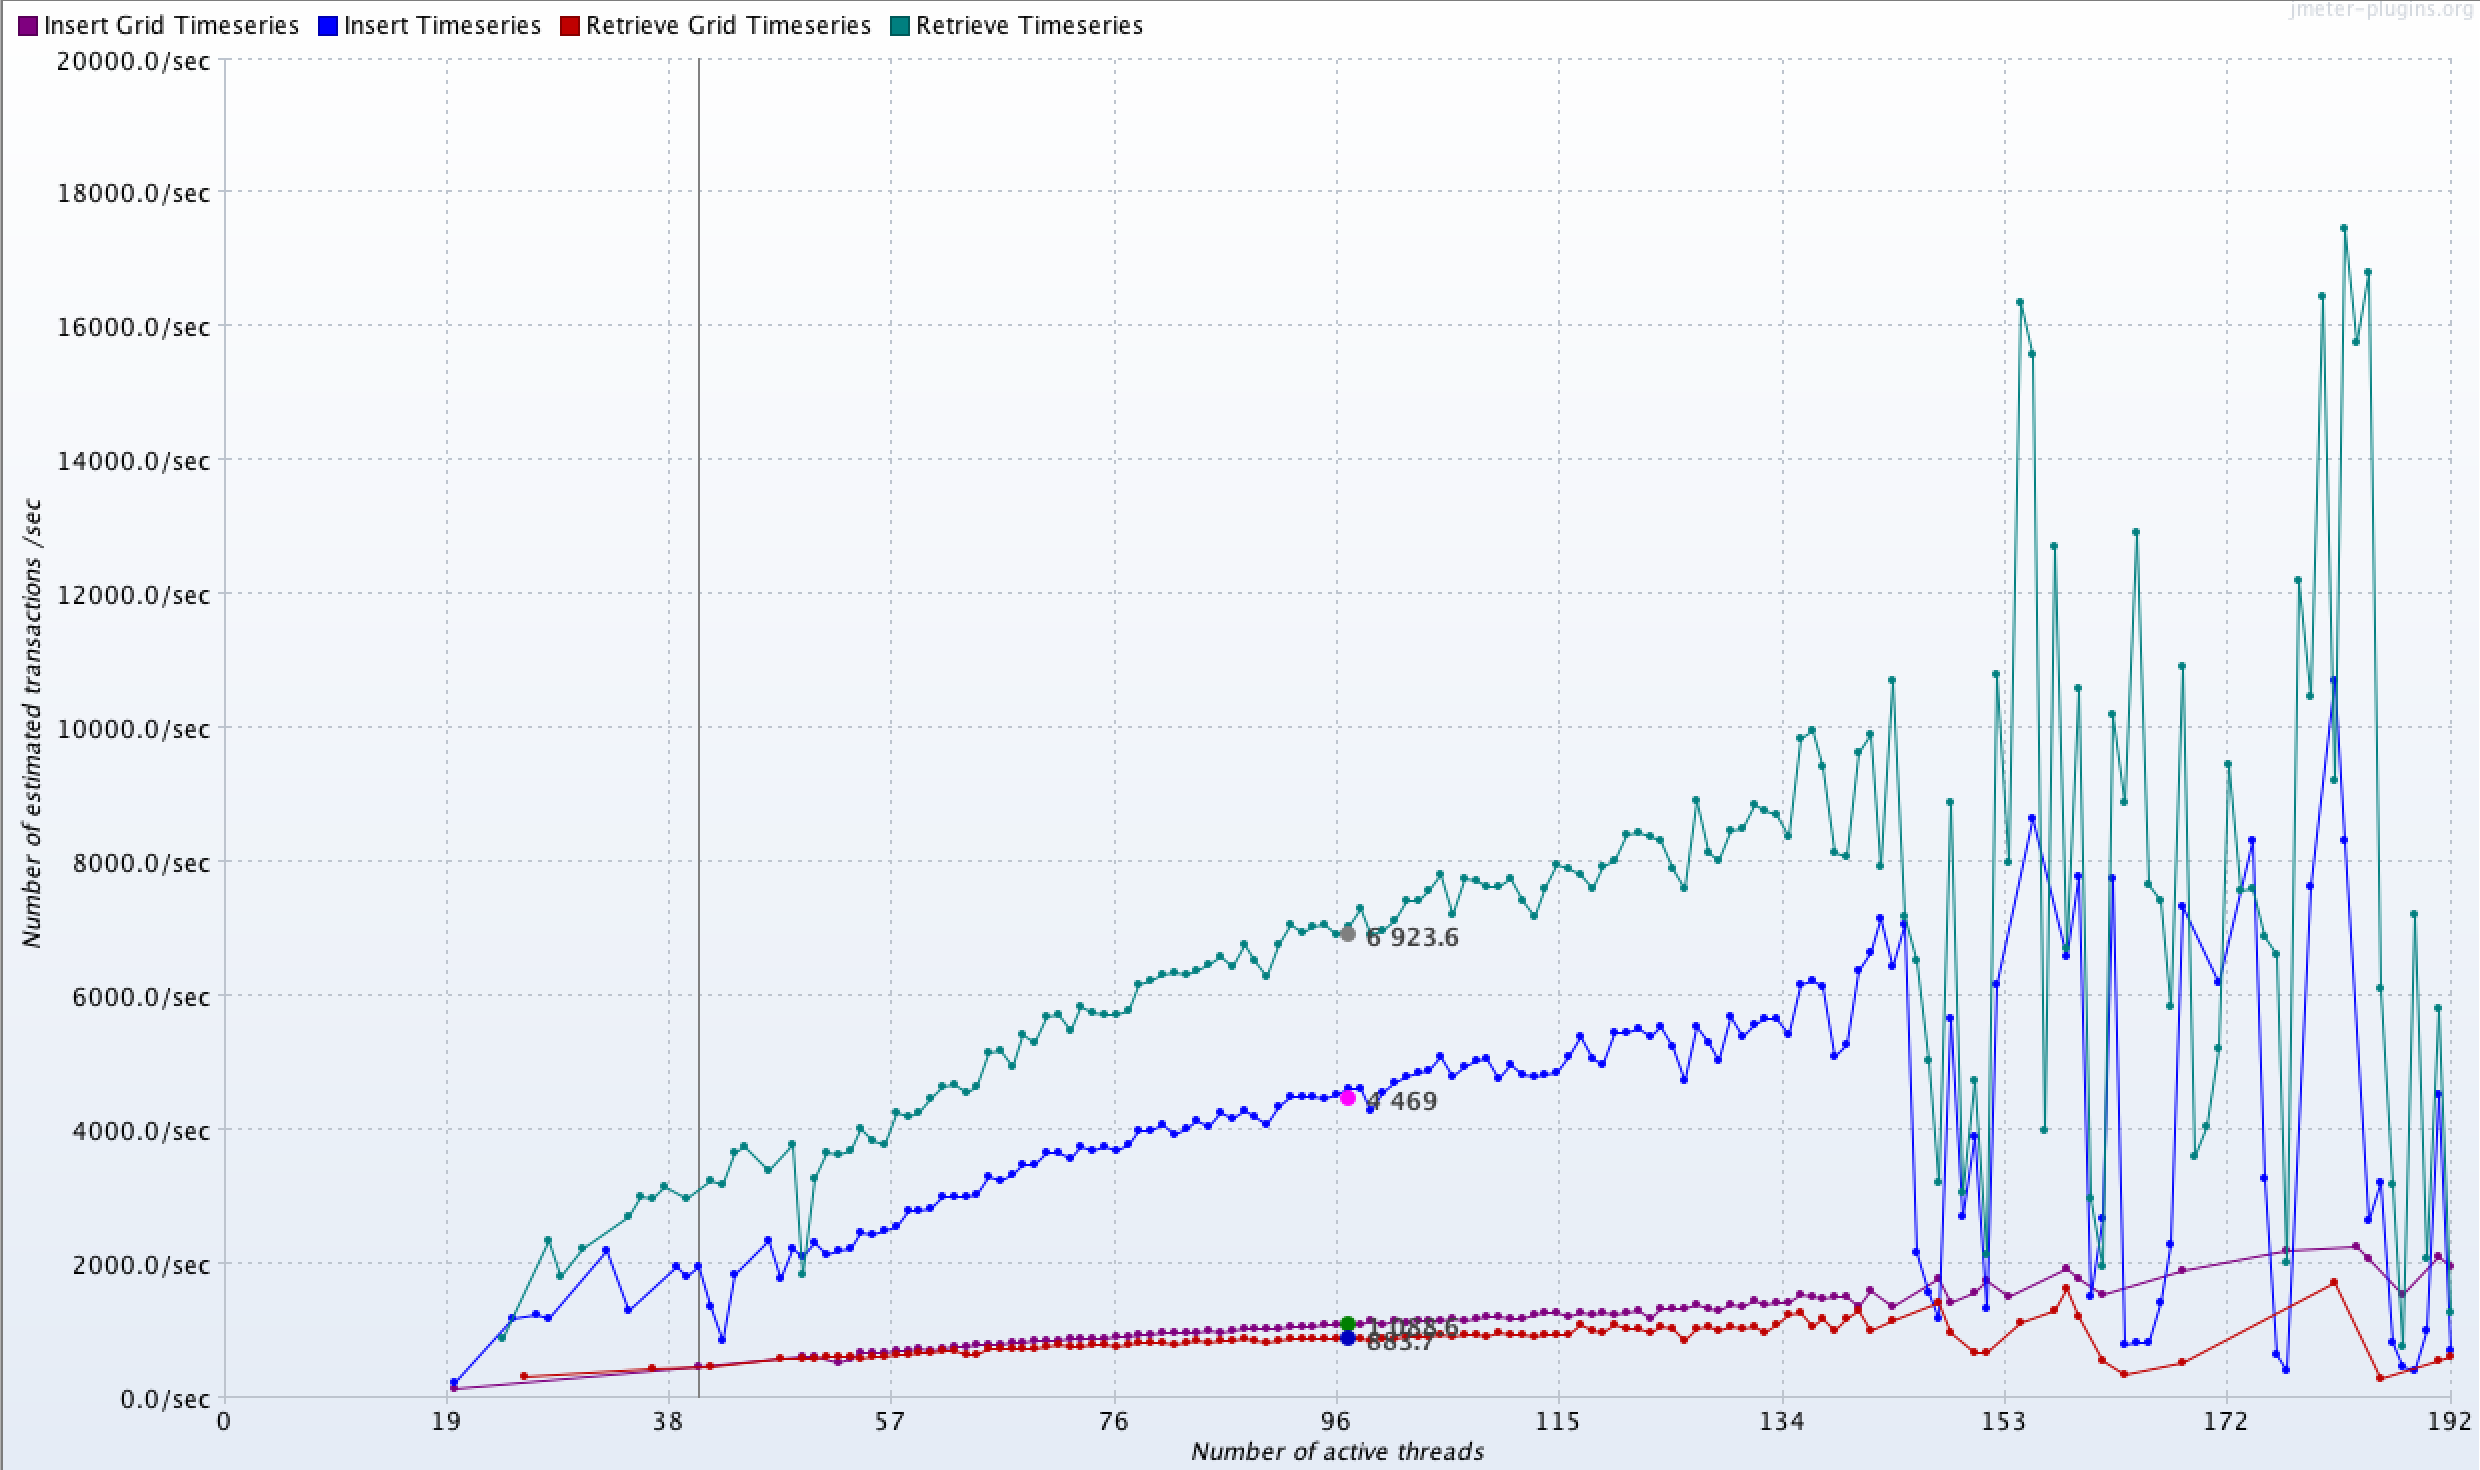
\includegraphics[width=0.8\textwidth]{results/obs/all/obs_all_15m_transaction_throughtput_vs_threads.png}
    \caption{Load testing with 15 minutes data - Transaction Throughput vs Threads}
    \label{fi:test_obs_all_15m_throughtput}
\end{figure}
\ref{fi:test_obs_all_15m_throughtput} shows the total server's transaction throughput against number of active threads.
The formula for total server transaction throughput is \(<active threads> * 1 second / <1  thread response time>\) \cite{JMeterPluginsTransactionPlugin}. Basically, it shows the statistical maximum possible number of transactions based on number of users accessing the application.
With combining the \ref{fi:test_obs_all_15m_latency}, this graph show that the throughput of the system get increased without much change in the latency, thus it proves the scalability of the \acrshort{wdias}.

\begin{figure}[htp]
    \centering
    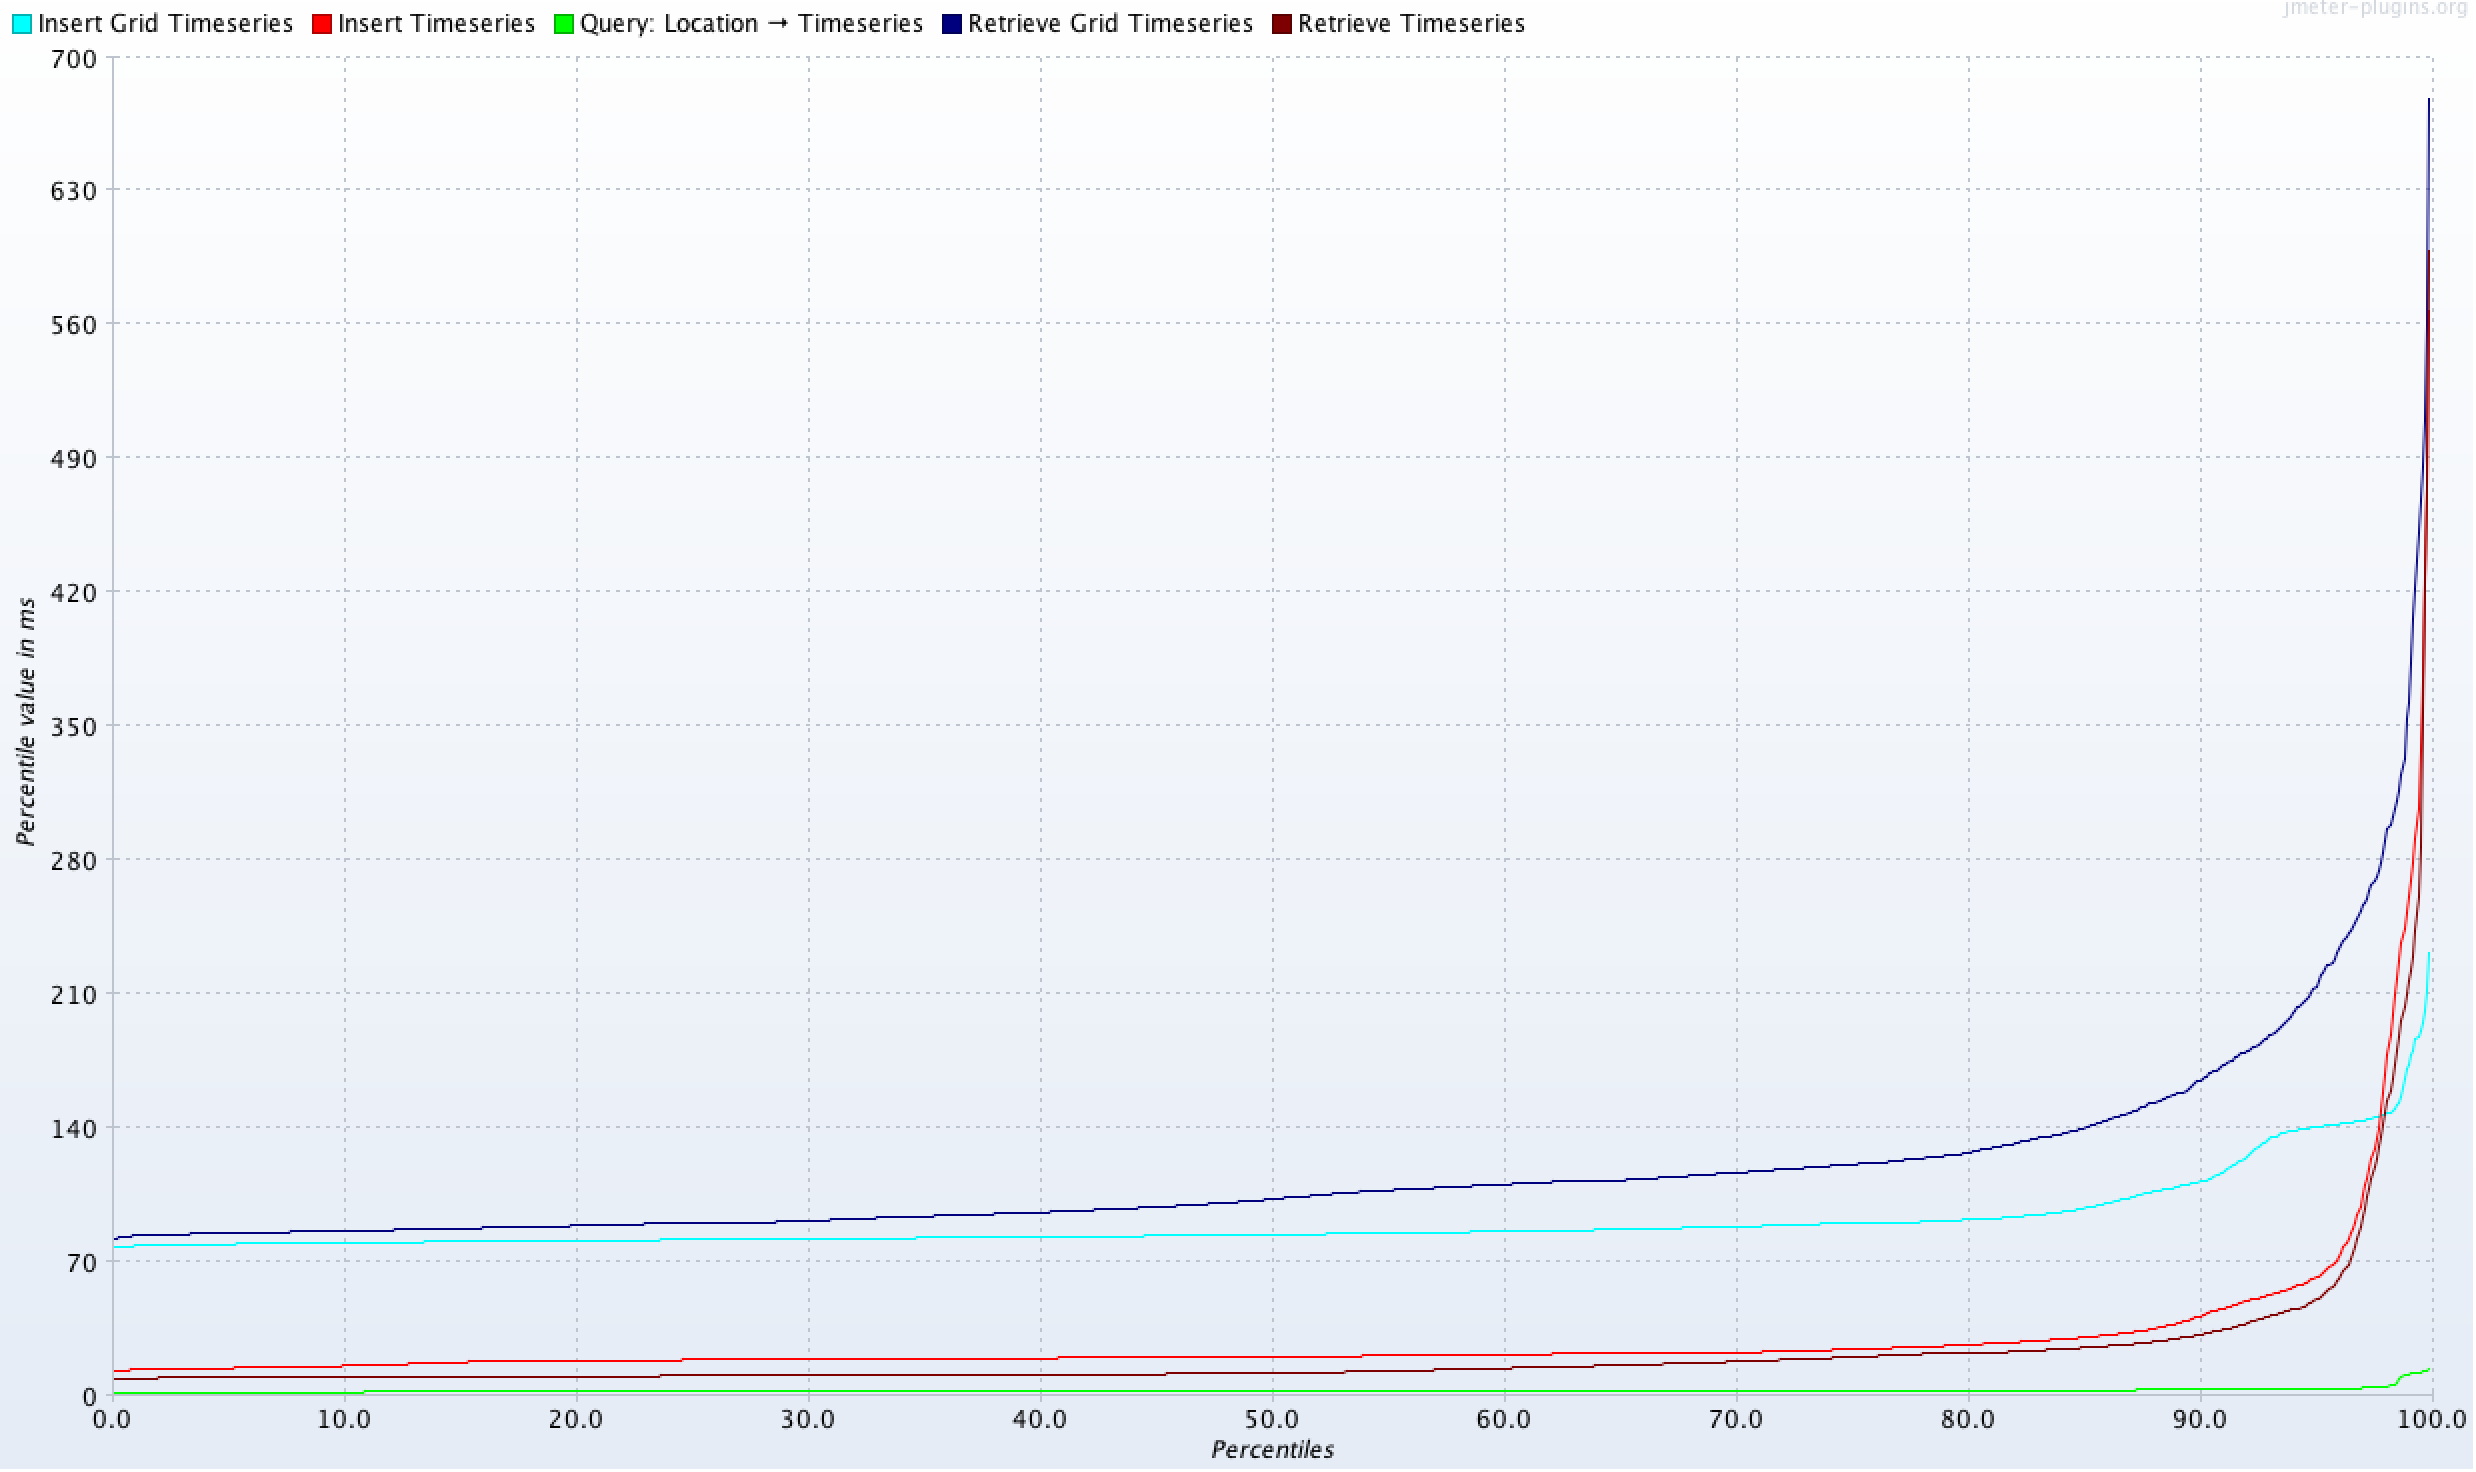
\includegraphics[width=0.8\textwidth]{results/obs/all/obs_all_15m_response_times_percentiles.png}
    \caption{Load testing with 15 minutes data - Response times Percentiles}
    \label{fi:test_obs_all_15m_latency_percentile}
\end{figure}
\ref{fi:test_obs_all_15m_latency_percentile} visually shows the summary of \ref{tab:obs_all_15_min_summary} latency up to 90\% percentile. With a higher request size data, the \acrshort{wdias} able to process the requests without significant change in latency up to 90\% percentile.


%%%%%%%%%%%%%%%%%%%%%%%%%%%%%%%%%%%%%%%%%%%%%%%%%%%%%%%%%%%%%%%%%%%%%%%%%%%%%%%%
\subsection{Load Testing with Auto Pod Scaling}
\label{subse:obs_test_plan_all_auto_15min}
This section \ref{subse:obs_test_plan_all_auto_15min} discussed about the All test plan performance with 15 minutes data which means 96 data points per each request in Scalar and Vector timeseries, and 96 ASCII Grid files per each insert Grid timeseries request. These requests are four times larger than the \ref{subse:obs_test_plan_all_60min} request size. It performed approximately 311k of sample requests which is almost similar to \ref{subse:obs_test_plan_all_15min} processed samples.
Other than that, this test plan runs with enabling \acrshort{k8s} Auto Scaling for the high resource utilized microservice as explained in the \ref{subse:test_plan_metrics}. With the test load used for the performance test, import-ascii-grid-upload microservice is using lots of CPU, and adapter-grid microservice is using lots of Memory. During this test plan, \acrshort{wdias} start with the auto scaling enabled for import-ascii-grid-upload microservice. Since adapter-grid is a consistence service for storing netCDF files, it is not possible to auto scale, since \acrshort{eks} does not support multiple read write support volumes \cite{LinuxFoundationPersistentKubernetes}.

\begin{table}[ht]
\caption{Throughput and Latency of load testing with 15min data while enabled \acrshort{k8s} Auto Scaling}
\footnotesize
\begin{tabulary}{\linewidth}{|L|C|C|C|C|C|C|C|C|}
\hline
Label & Samples & Avg & Min & Max & 90\% Line & Std. Dev. & Error \% & RPS \\ \hline
Insert Timeseries & 71727 & 34 & 13 & 1777 & 27 & 118.78 & 0.00\% & 40.5 \\ \hline
Retrieve Timeseries & 71693 & 7 & 5 & 1608 & 9 & 18.72 & 0.00\% & 40.5 \\ \hline
Insert Grid & 7968 & 87 & 77 & 233 & 98 & 14.07 & 0.18\% & 4.5 \\ \hline
Retrieve Grid & 7965 & 89 & 63 & 1694 & 110 & 37.79 & 0.00\% & 4.5 \\ \hline
Query: Location & 71704 & 1 & 0 & 203 & 2 & 2.05 & 0.00\% & 40.5 \\ \hline
\textbf{TOTAL} & 310734 & 130 & 0 & 1777 & 501 & 212.35 & 0.00\% & 175.3 \\ \hline
\end{tabulary}
\label{tab:obs_all_auto_15_min_summary}
\end{table}
\ref{tab:obs_all_auto_15_min_summary} shows the response latency summary details and \acrshort{rps} as same as explained in \ref{subse:obs_test_plan_all_15min}.
During this test plan. the main focus on the auto scaling enabled microservice. As per the insert grid latency in the \ref{tab:obs_all_auto_15_min_summary}, the average insert latency is reduced from 91ms to 87ms. Also error percentage reduced from 1.42\% to 0.18\%. Standard deviation reduced from 19.58 to 14.07 which means the latency is much closer to the average latency. These improvements in insert Grid timeseries data seems to affect on out put of retrieve Grid timeseries data as well.

\begin{figure}[htp]
    \centering
    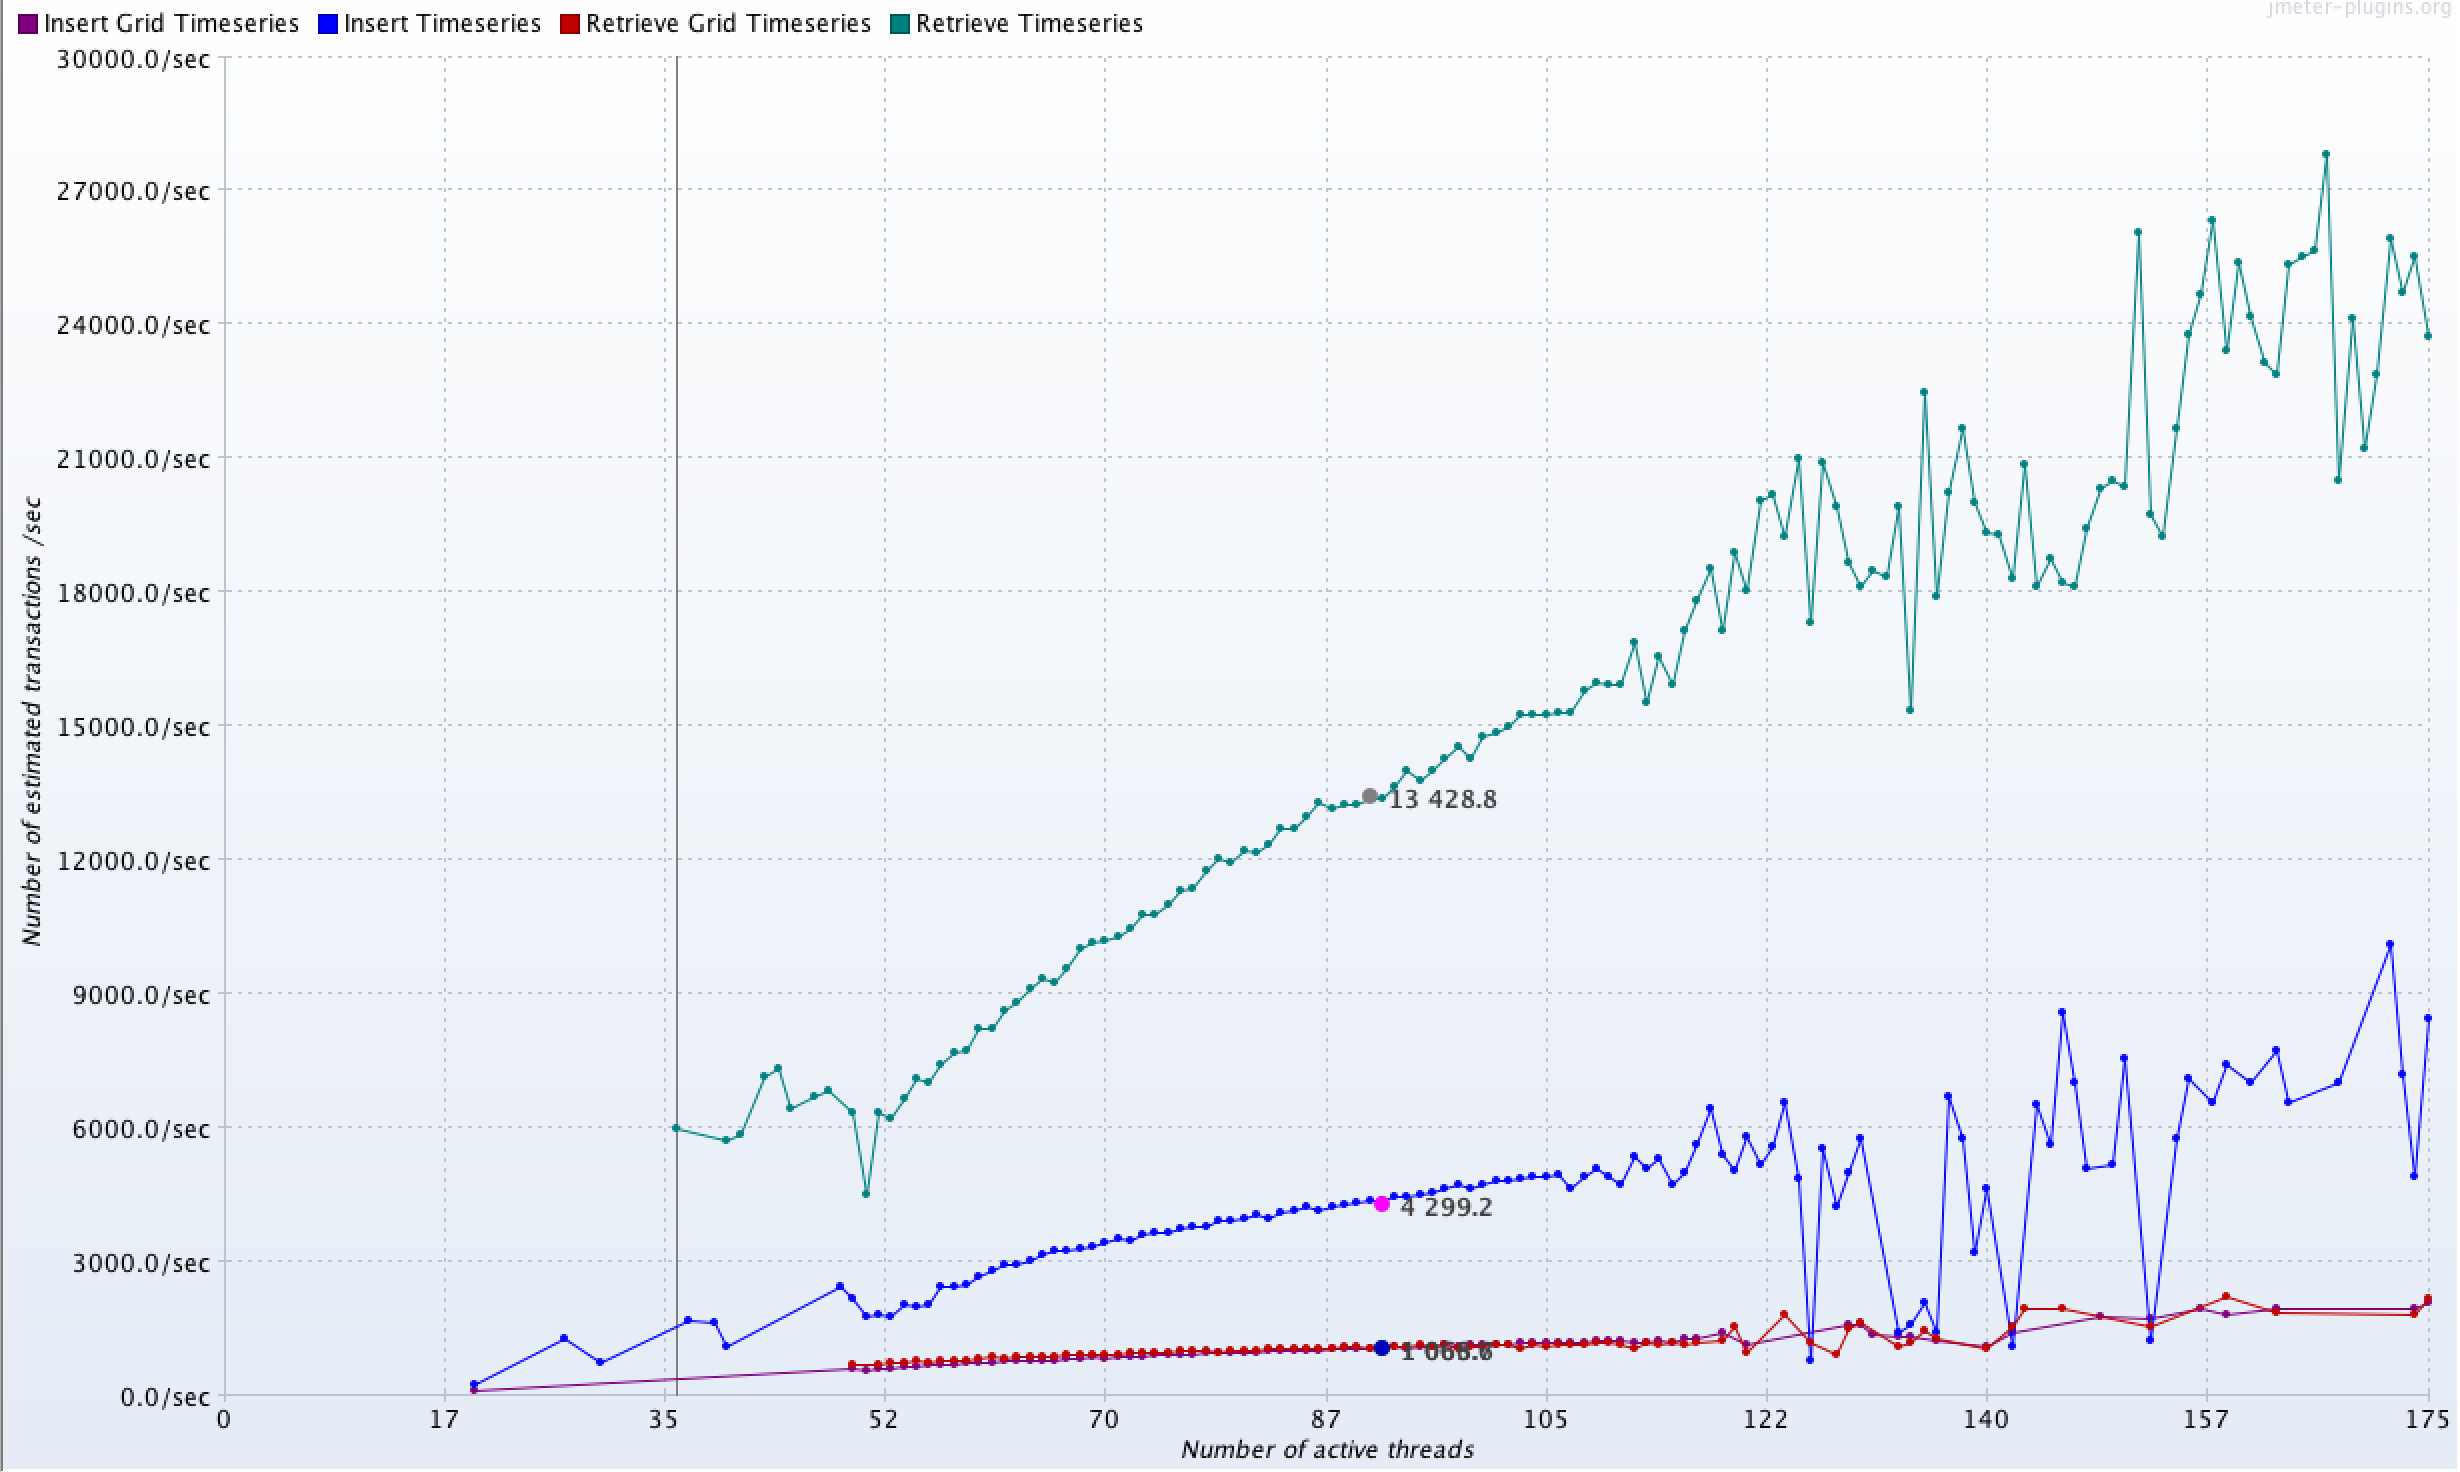
\includegraphics[width=0.8\textwidth]{results/obs/all_auto/obs_all_auto_15m_transaction_throughtput_vs_threads.png}
    \caption{Load testing with 15 minutes data with enabled auto scaling - Latency against server hits}
    \label{fi:test_obs_all_auto_15m_latency}
\end{figure}
\ref{fi:test_obs_all_auto_15m_latency} graph provides an overview of the variation of latency over elapsed time of the test plan against number of server hits per second for 15min data while auto scaling enabled for \acrshort{k8s}.
This graph show that over the time \acrshort{wdias} were able to keep the latency constant over the test plan.
When compared to \ref{fi:test_obs_all_15m_latency}, throw out the test time period, the latency spikes become less.

\begin{figure}[htp]
    \centering
    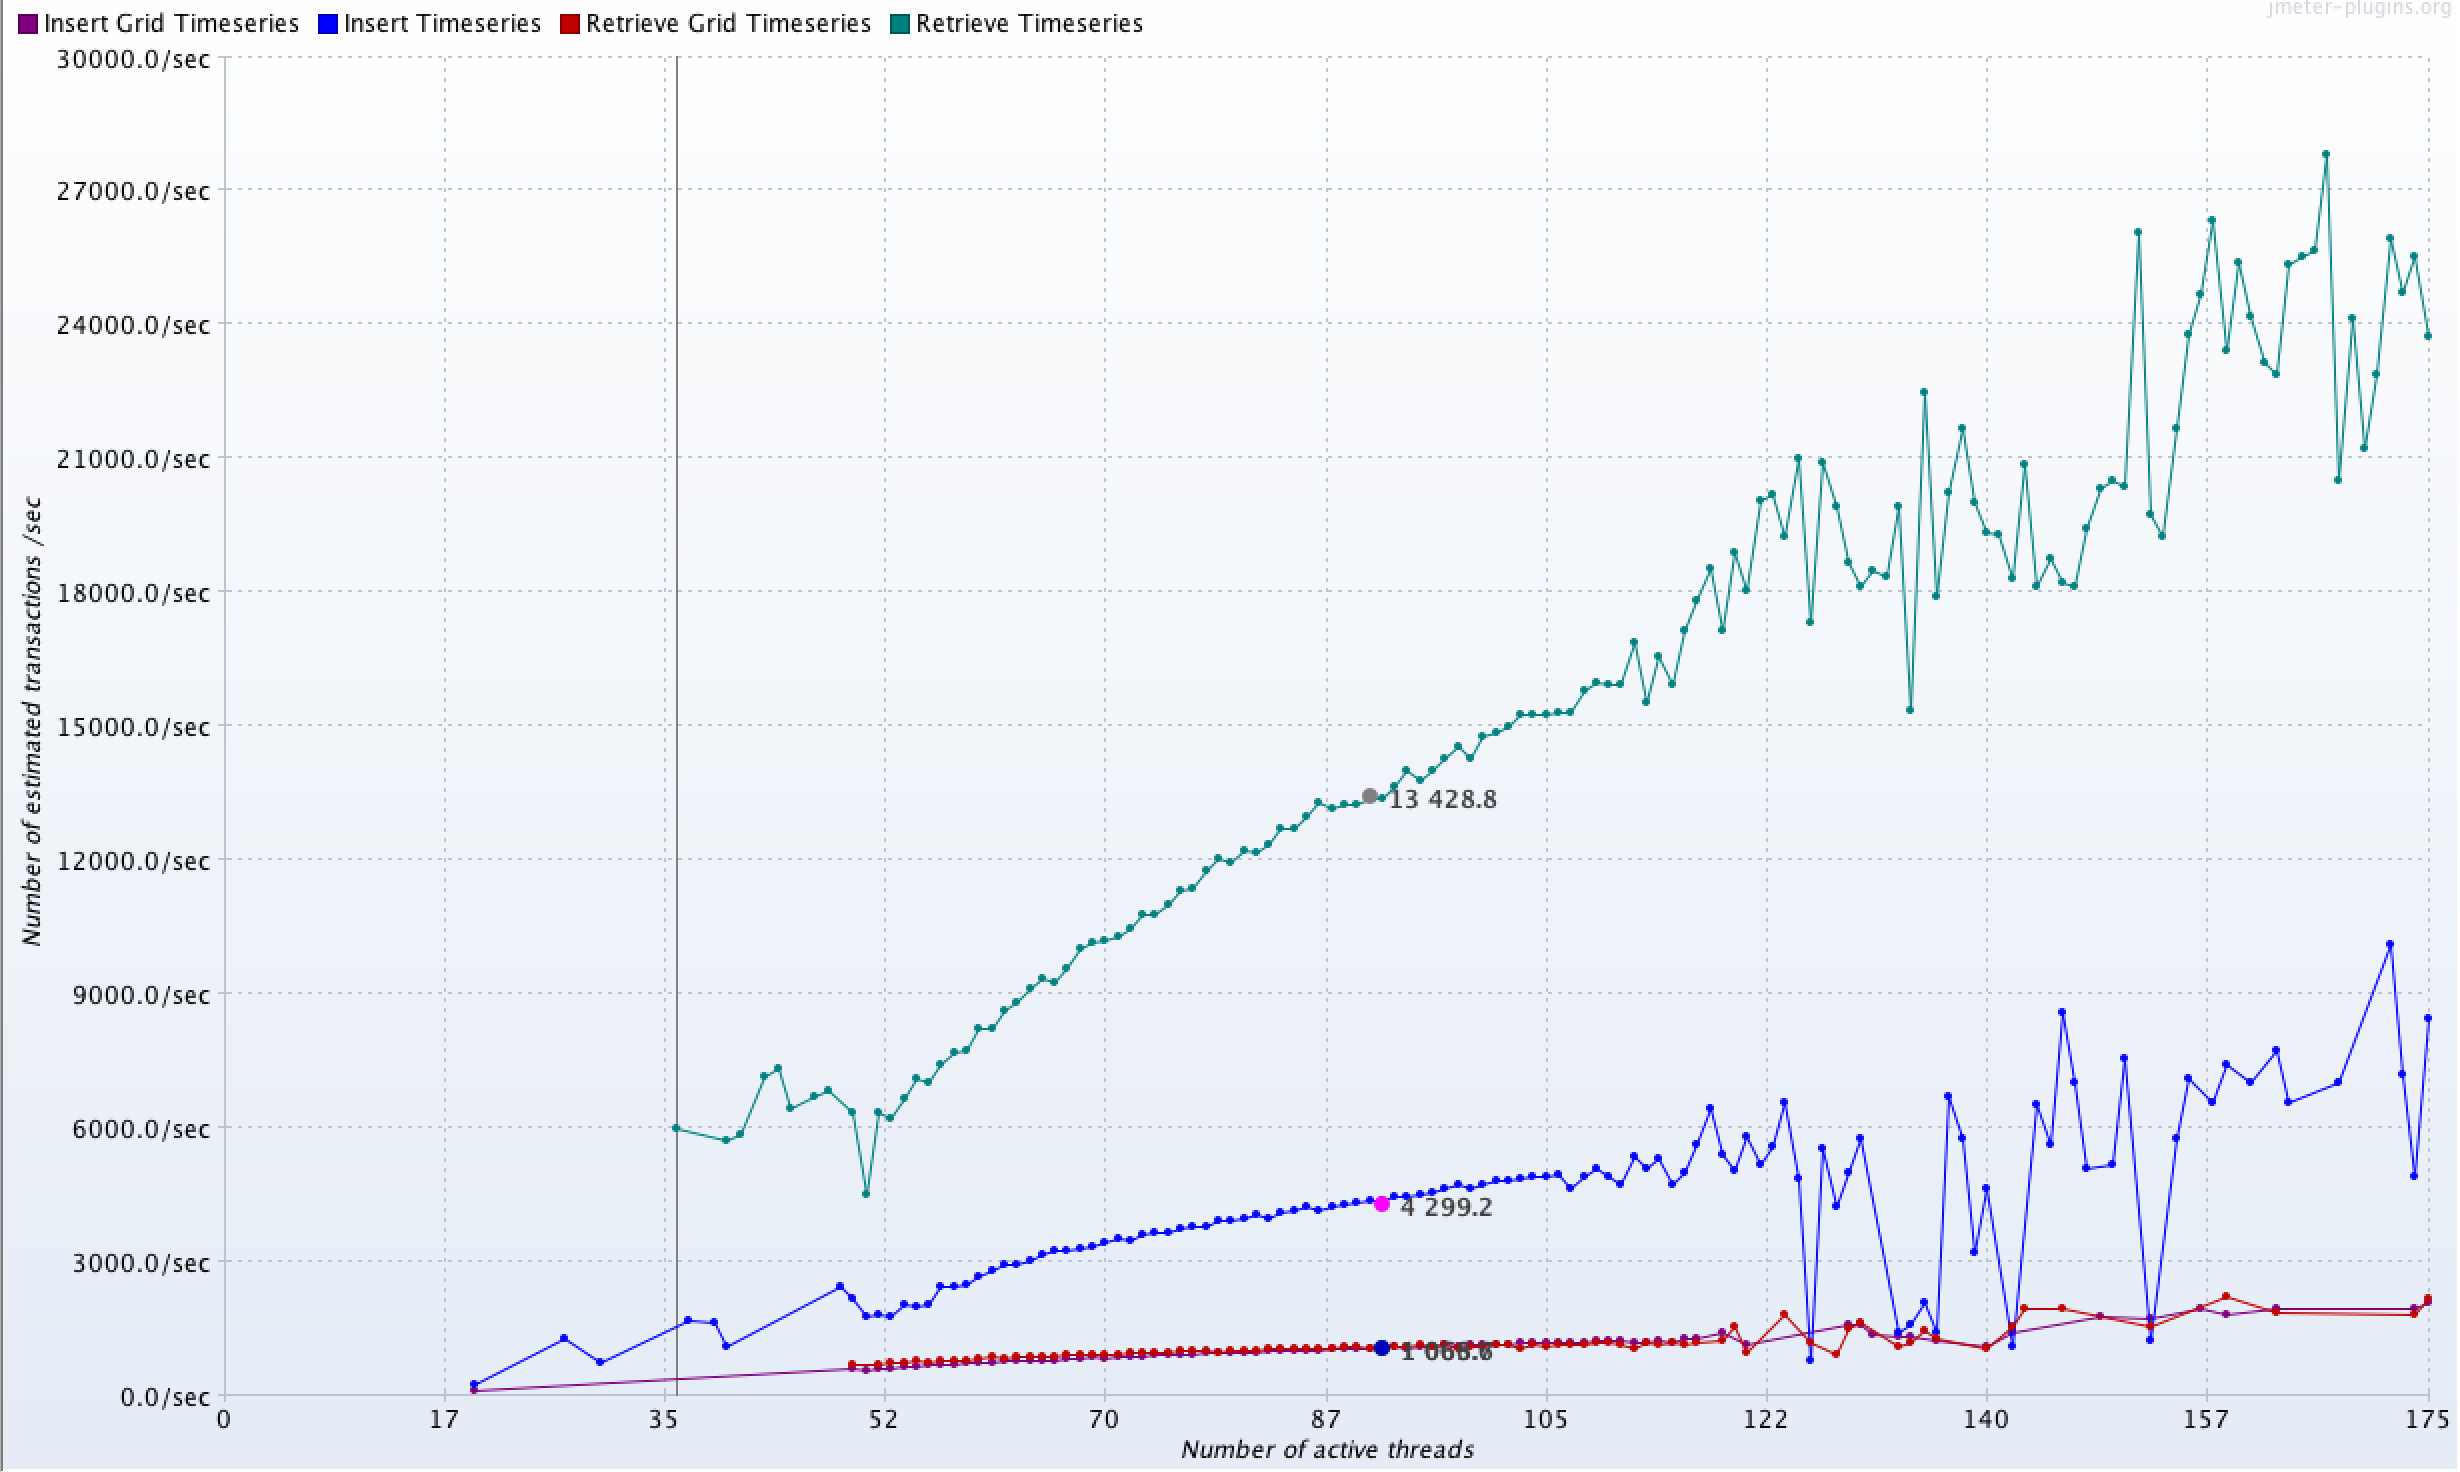
\includegraphics[width=0.8\textwidth]{results/obs/all_auto/obs_all_auto_15m_transaction_throughtput_vs_threads.png}
    \caption{Load testing with 15 minutes data with enabled auto scaling - Transaction Throughput vs Threads}
    \label{fi:test_obs_all_auto_15m_throughtput}
\end{figure}
\ref{fi:test_obs_all_auto_15m_throughtput} shows the total server's transaction throughput against number of active threads.
When compared to \ref{fi:test_obs_all_15m_throughtput}, estimated throughput with higher number of active threads become stable at the graph. Which means enabling auto scaling improve the throughput with higher number of active users as well.

Following charts show the resource usage while running the all test plan while enabling the auto scaling.
\begin{figure}[htp]
    \centering
    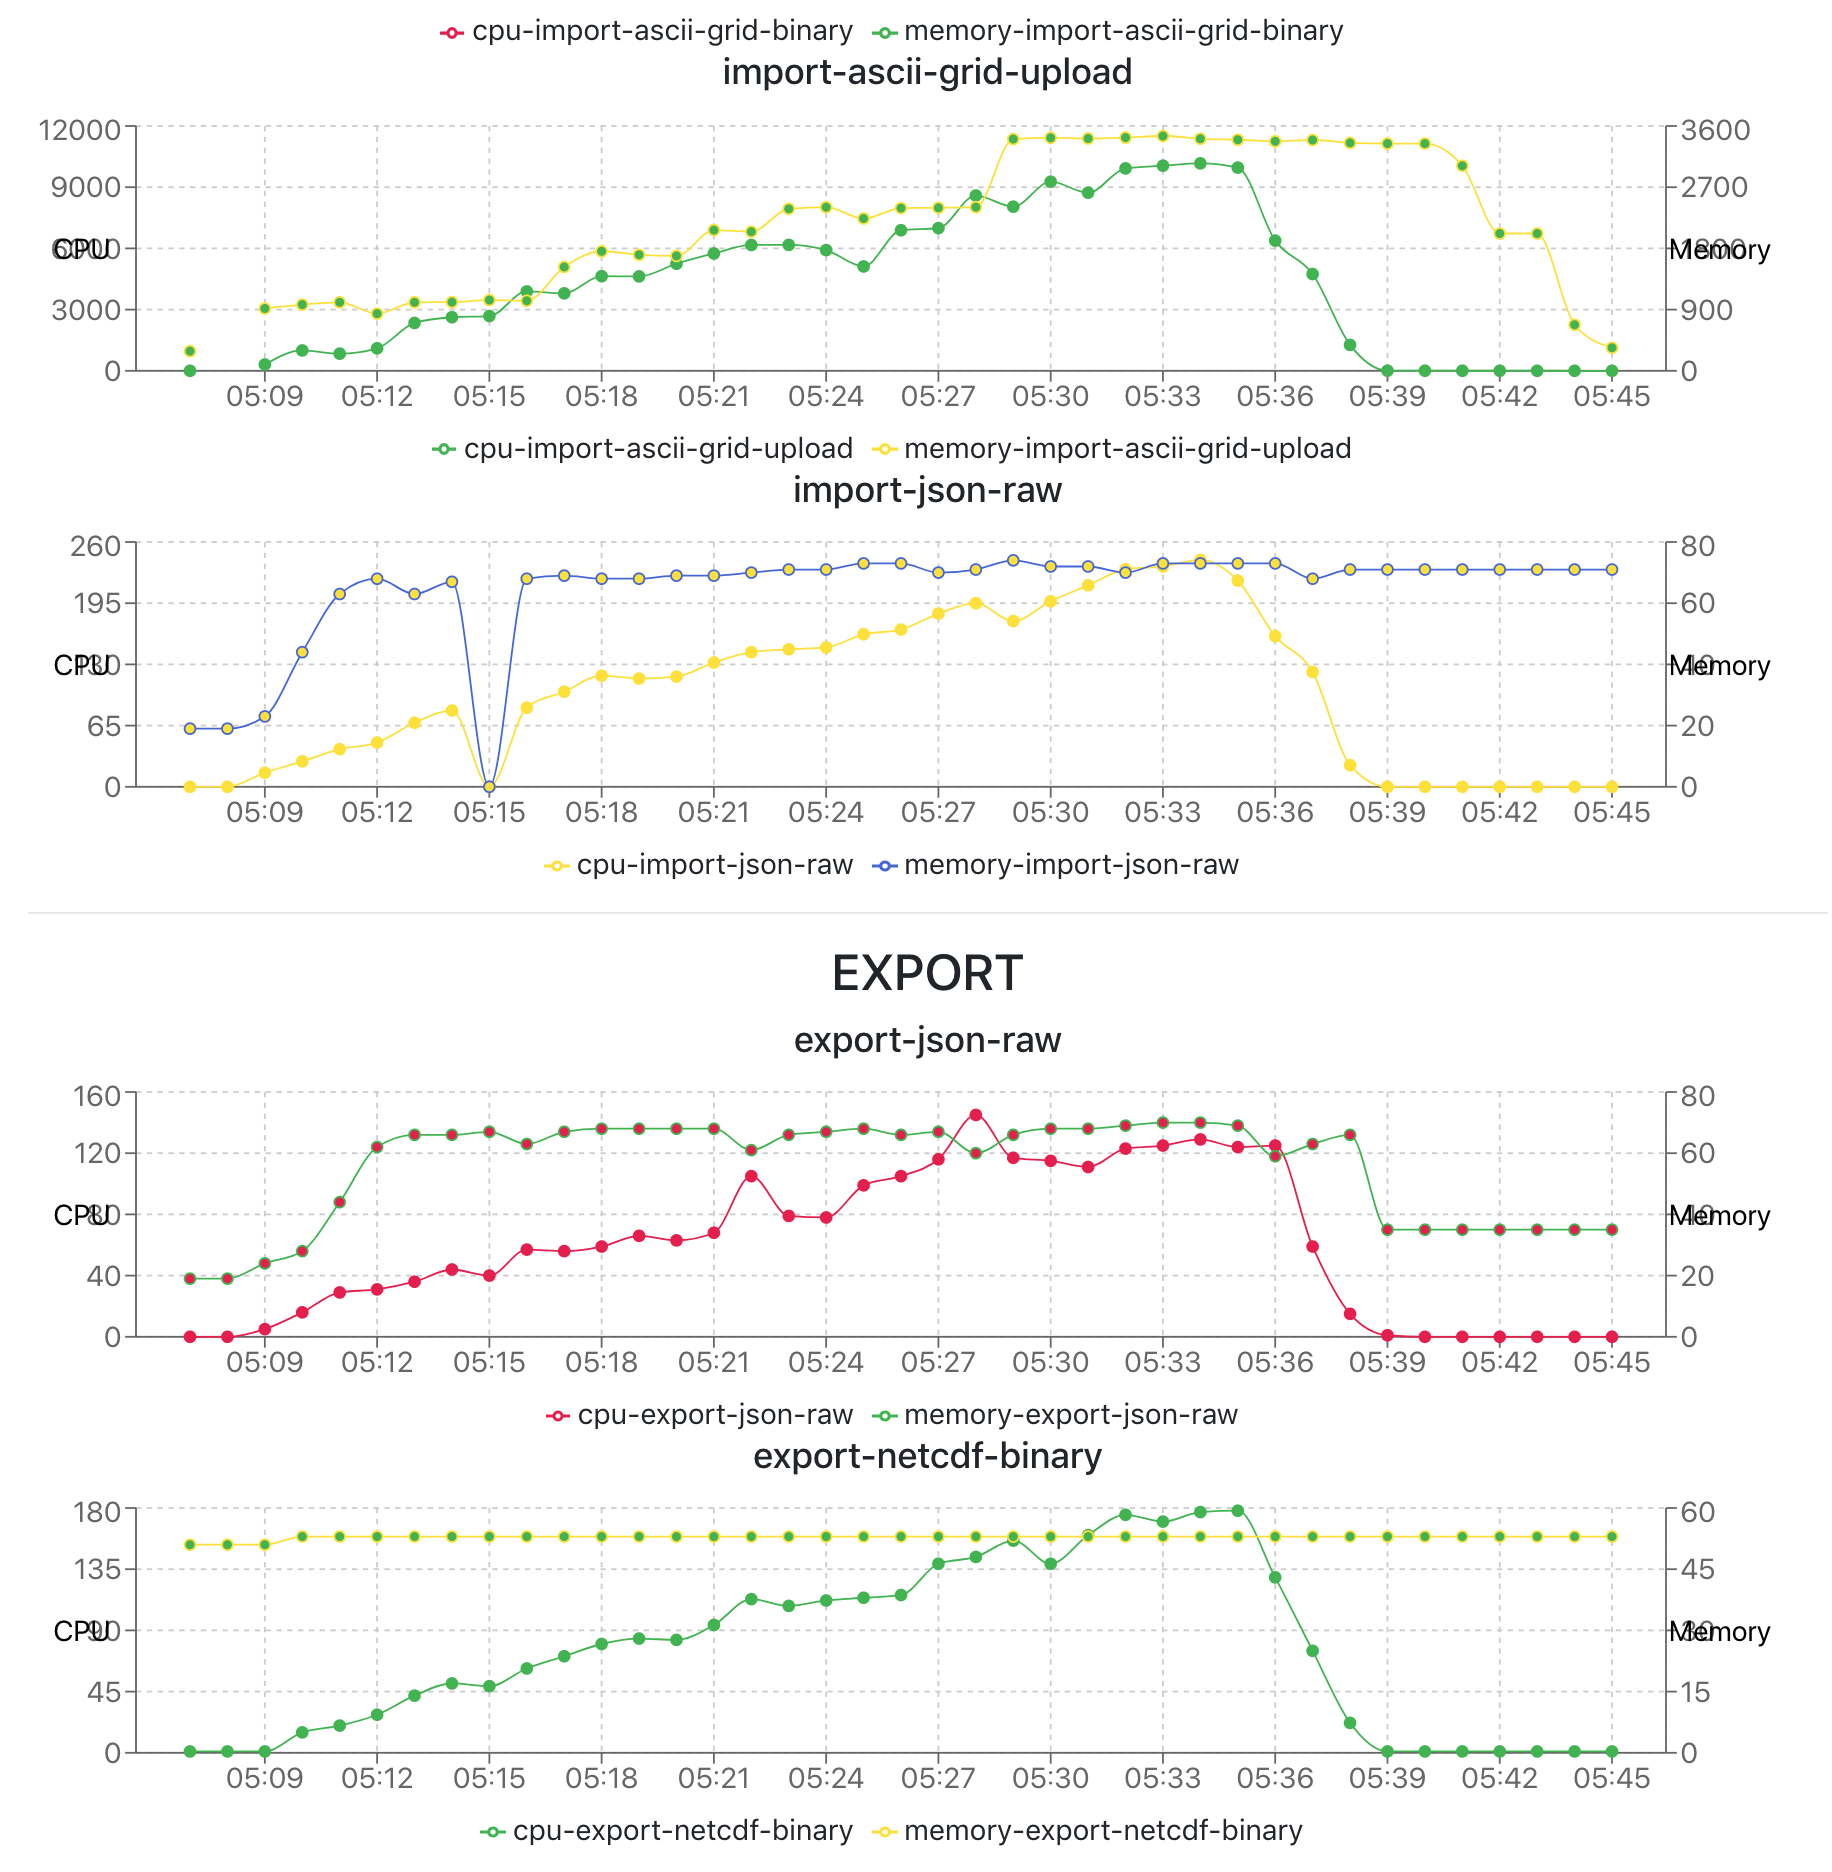
\includegraphics[width=0.8\textwidth]{results/obs/all_auto/obs_all_auto_15m_import_export_res.png}
    \caption{Load testing with auto scaling resource usage of import and export modules.}
    \label{fi:obs_all_auto_15m_import_export_res}
\end{figure}
\ref{fi:obs_all_auto_15m_import_export_res} show the CPU usage and Memory usage for import timeseries modules and export timeseries modules. The CPU usage shown with milli CPUs \cite{LinuxFoundationManagingKubernetes} (1 CPU = 1000m CPUs) and the Memory usage shown with Megabytes (Mi) \cite{LinuxFoundationManagingKubernetes}. Noticeable, the import-ascii-grid-upload microservice used around 10 CPUs at the peak time while using 3.6 Gb of Memory. Another important fact is, after the test cases finished, the \acrshort{wdias} cool down the system via \acrshort{k8s} auto scaling and release the resources. This clearly shows the elasticity of the \acrshort{wdias} according to the workload.

\begin{figure}[htp]
    \centering
    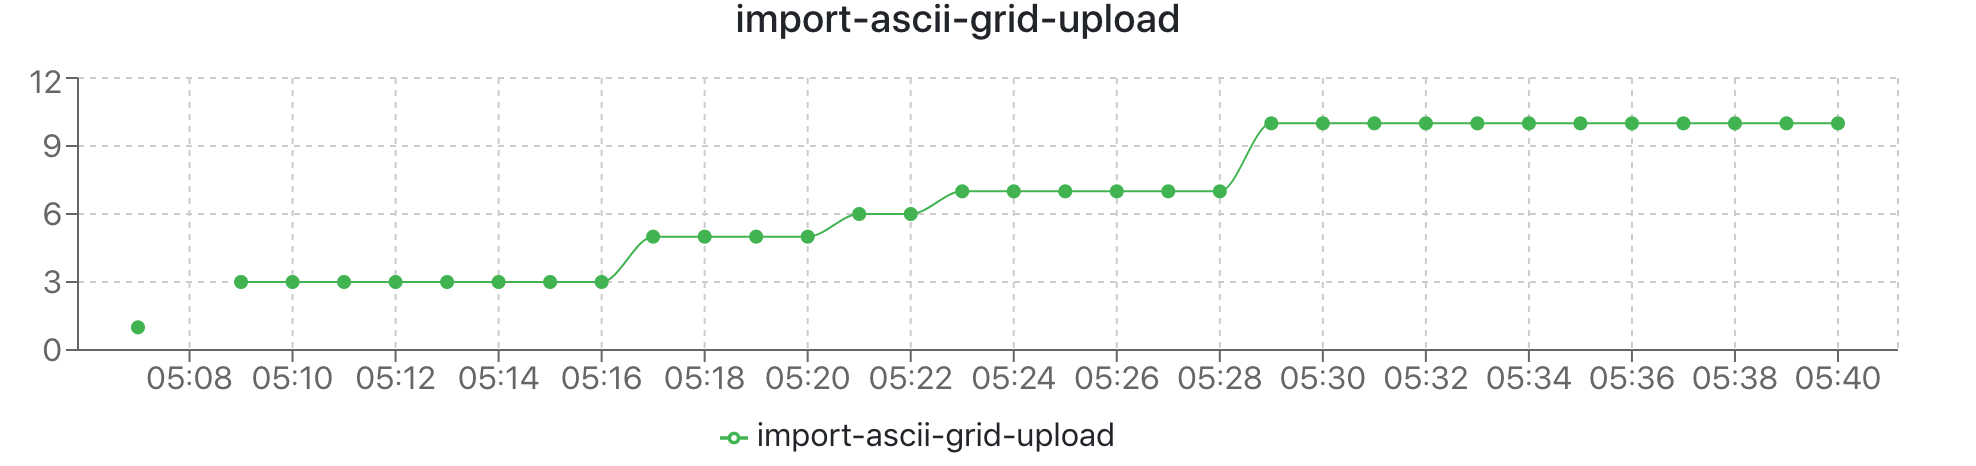
\includegraphics[width=0.8\textwidth]{results/obs/all_auto/obs_all_auto_15m_import_grid_pod.png}
    \caption{Load testing with auto scaling import ascii grid number of pods over time.}
    \label{fi:obs_all_auto_15m_import_grid_pod}
\end{figure}
\ref{fi:obs_all_auto_15m_import_grid_pod} shows the number of import-ascii-grid-upload pods scheduled over time. The auto scaling enabled with the configurations of 1 to 10 pods with the recommended CPU usage with 80\%. And the pods scheduled with 1 CPU requested, and limit with 2 CPUs per pod.
As the graph shows, 3 pods scheduled at the initial as per the configuration of the helm chart. While increasing the workload, new pods get spawn while keeping the constraint of 80\% of recommended CPU utilization. After \acrshort{k8s} spawn 10 maximum pods, it stop spawning new pods. But the pods were able to perform with vertical scaling, since those are not hit the CPU limit of 2.

\begin{figure}[htp]
    \centering
    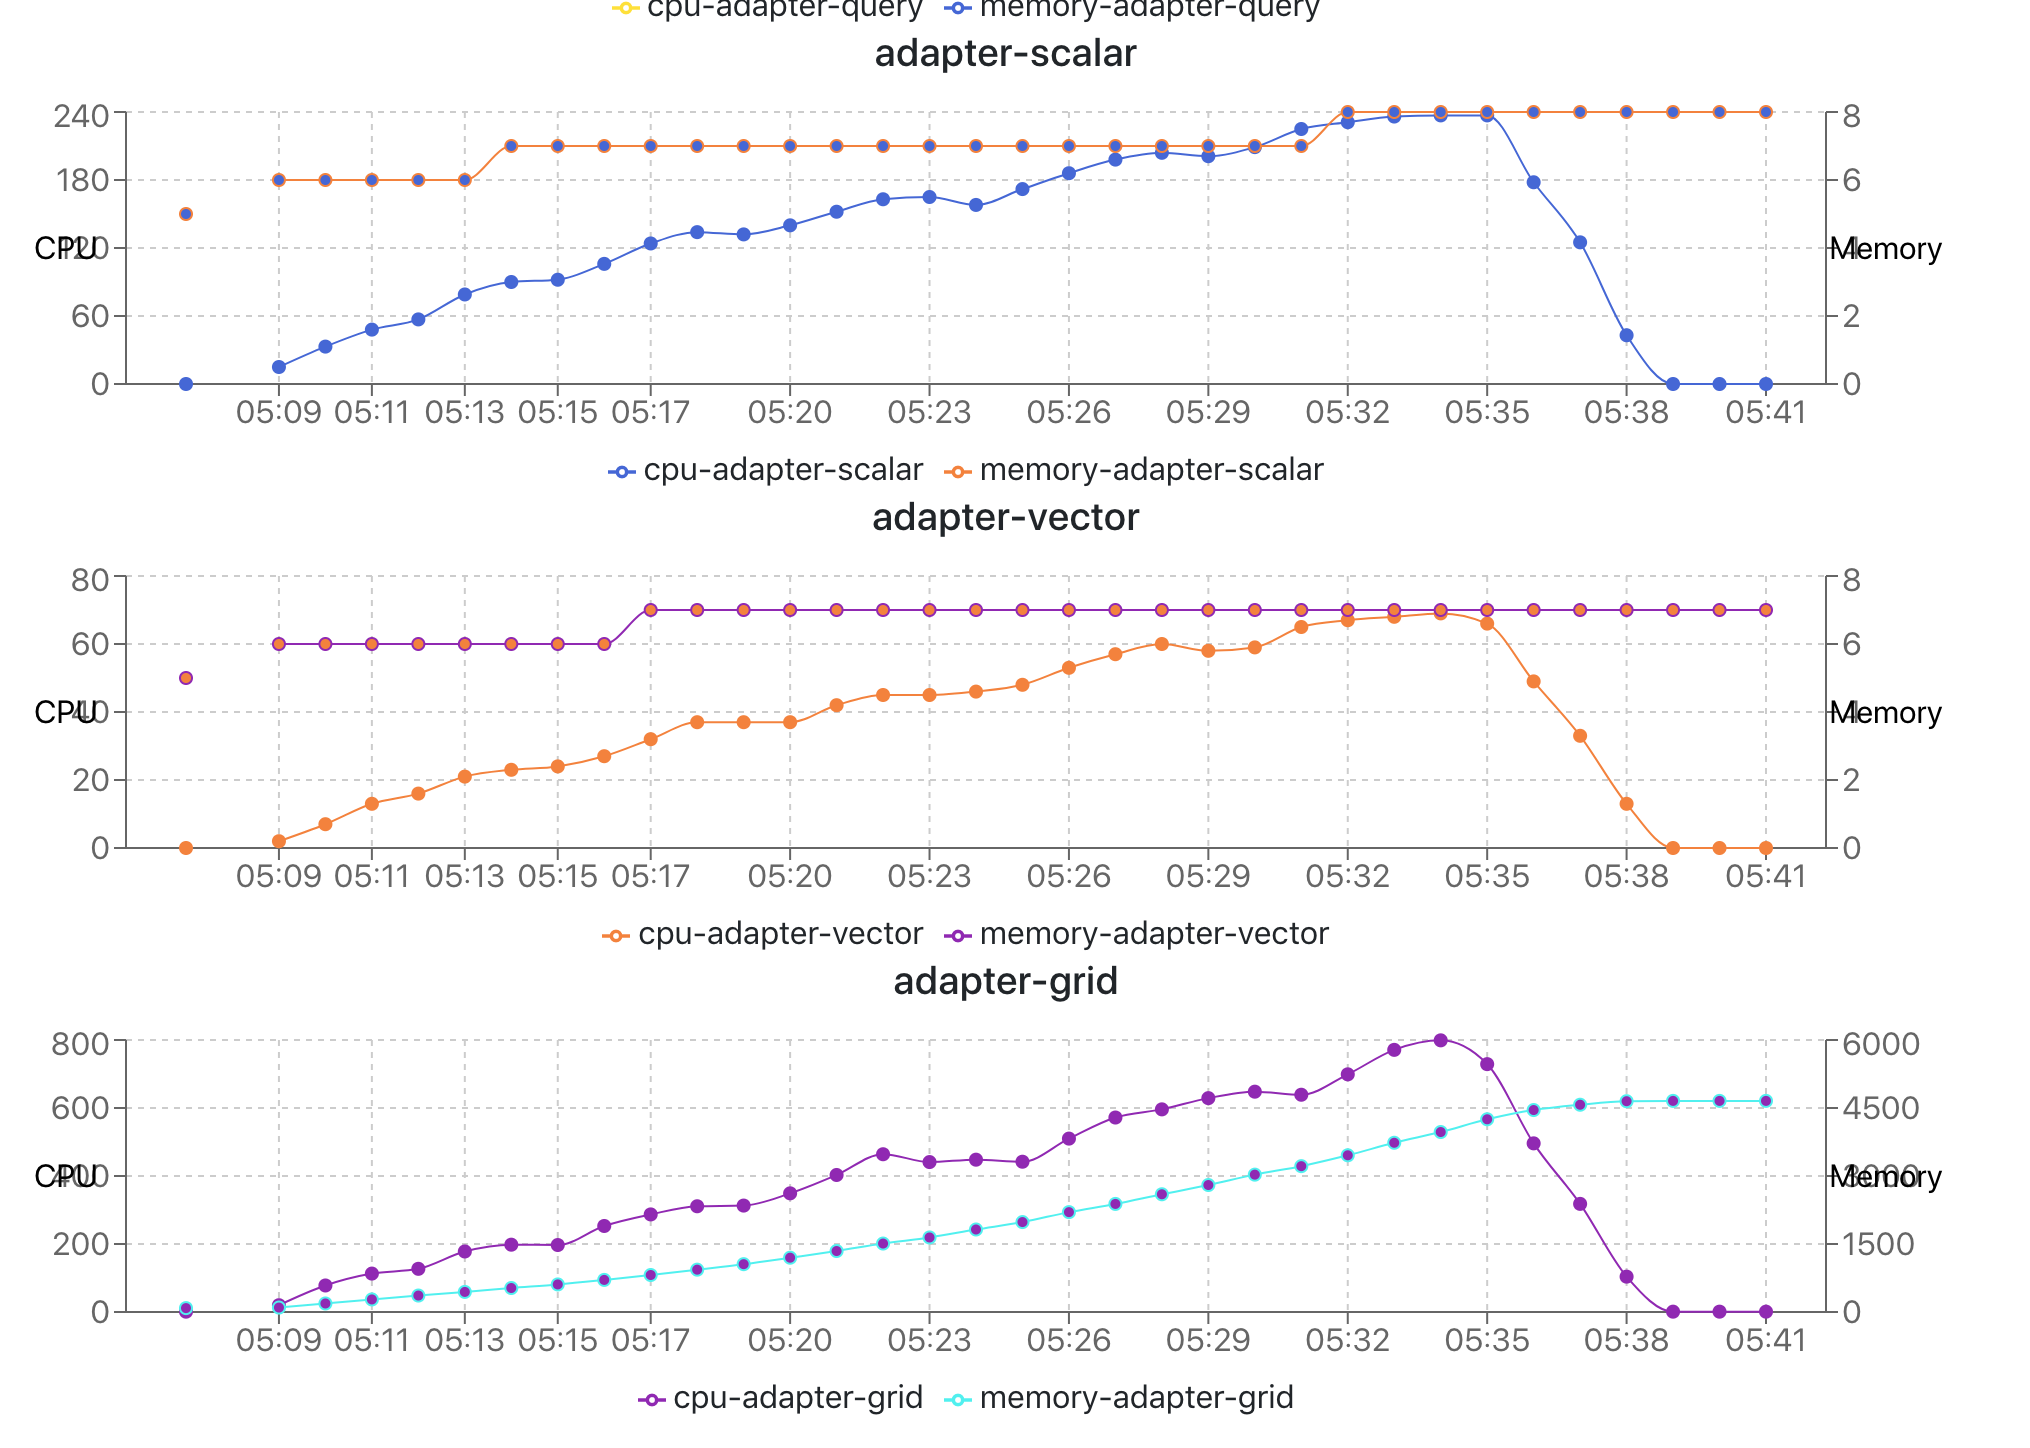
\includegraphics[width=0.8\textwidth]{results/obs/all_auto/obs_all_auto_15m_adapter_dbs_res.png}
    \caption{Load testing with auto scaling resource usage of database adapters.}
    \label{fi:obs_all_auto_15m_adapter_dbs_res}
\end{figure}
\ref{fi:obs_all_auto_15m_adapter_dbs_res} shows the resource utilization of database adapters in the \acrshort{wdias}.


%%%%%%%%%%%%%%%%%%%%%%%%%%%%%%%%%%%%%%%%%%%%%%%%%%%%%%%%%%%%%%%%%%%%%%%%%%%%%%%%
\subsection{Query Module Load Test}
\label{subse:obs_test_plan_query_15min}
This section \ref{subse:obs_test_plan_query_15min} discussed about the Query test plan performance. It performs multiple information retrieval queries such as query over locations, parameters and timeseries etc which are described over \ref{se:query}. It performed approximately 123k of sample requests.
Query test plan perform over 5 minutes of time period, and with a higher number of requests than other test plan with a peak of 600 hits per seconds.

\begin{table}[ht]
\caption{Throughput and Latency of Query test cases with 15min data}
\footnotesize
\begin{tabulary}{\linewidth}{|L|C|C|C|C|C|C|C|C|}
\hline
Label & Samples & Avg & Min & Max & 90\% Line & Std. Dev. & Error \% & RPS \\ \hline
* → Locations & 11462 & 992 & 5 & 17569 & 1740 & 704.67 & 0.00\% & 38.3 \\ \hline
Area → Locations & 11390 & 599 & 2 & 16755 & 1047 & 514.68 & 0.00\% & 38.1 \\ \hline
Location → Parameters & 11350 & 666 & 1 & 16821 & 1179 & 632.86 & 0.00\% & 38.0 \\ \hline
Locations → Parameters & 11305 & 659 & 1 & 17459 & 1149 & 678.55 & 0.00\% & 37.8 \\ \hline
Location → Timeseries & 11269 & 647 & 2 & 32693 & 1102 & 746.51 & 0.00\% & 37.7 \\ \hline
Locations → Timeseries & 11237 & 669 & 1 & 32651 & 1162 & 889.18 & 0.00\% & 37.6 \\ \hline
Locations, Parameter → Timeseries & 11192 & 662 & 2 & 32806 & 1152 & 789.49 & 0.00\% & 37.4 \\ \hline
Area → Timeseries & 11135 & 820 & 2 & 33235 & 1461 & 877.68 & 0.00\% & 37.3 \\ \hline
Area, Parameter → Timeseries & 11084 & 864 & 1 & 16699 & 1584 & 751.00 & 0.00\% & 37.1 \\ \hline
*, Parameter → Timeseries & 11011 & 696 & 2 & 16689 & 1216 & 693.33 & 0.00\% & 36.8 \\ \hline
* → Timeseries & 10968 & 1473 & 24 & 18283 & 2467 & 912.45 & 0.00\% & 36.7 \\ \hline
\textbf{TOTAL} & 123403 & 794 & 1 & 33235 & 1536 & 789.76 & 0.00\% & 412.6 \\ \hline
\end{tabulary}
\label{tab:obs_query_15_min_summary}
\end{table}
\ref{tab:obs_query_15_min_summary} shows the response latency summary details. The average latency is much higher than the minimum value. Also it reported higher maximum values as well. Standard deviation showed as quiet higher value which means the response latency values are not closer to the average value. Noticeably, it does not reported any errors, which means all the requests successfully process.
The throughput for each test case is much higher and similar to all the requests. This is happening since all of these requests are handle via the adapter-query, it depends on the \acrshort{mongodb} database performance.

\begin{figure}[htp]
    \centering
    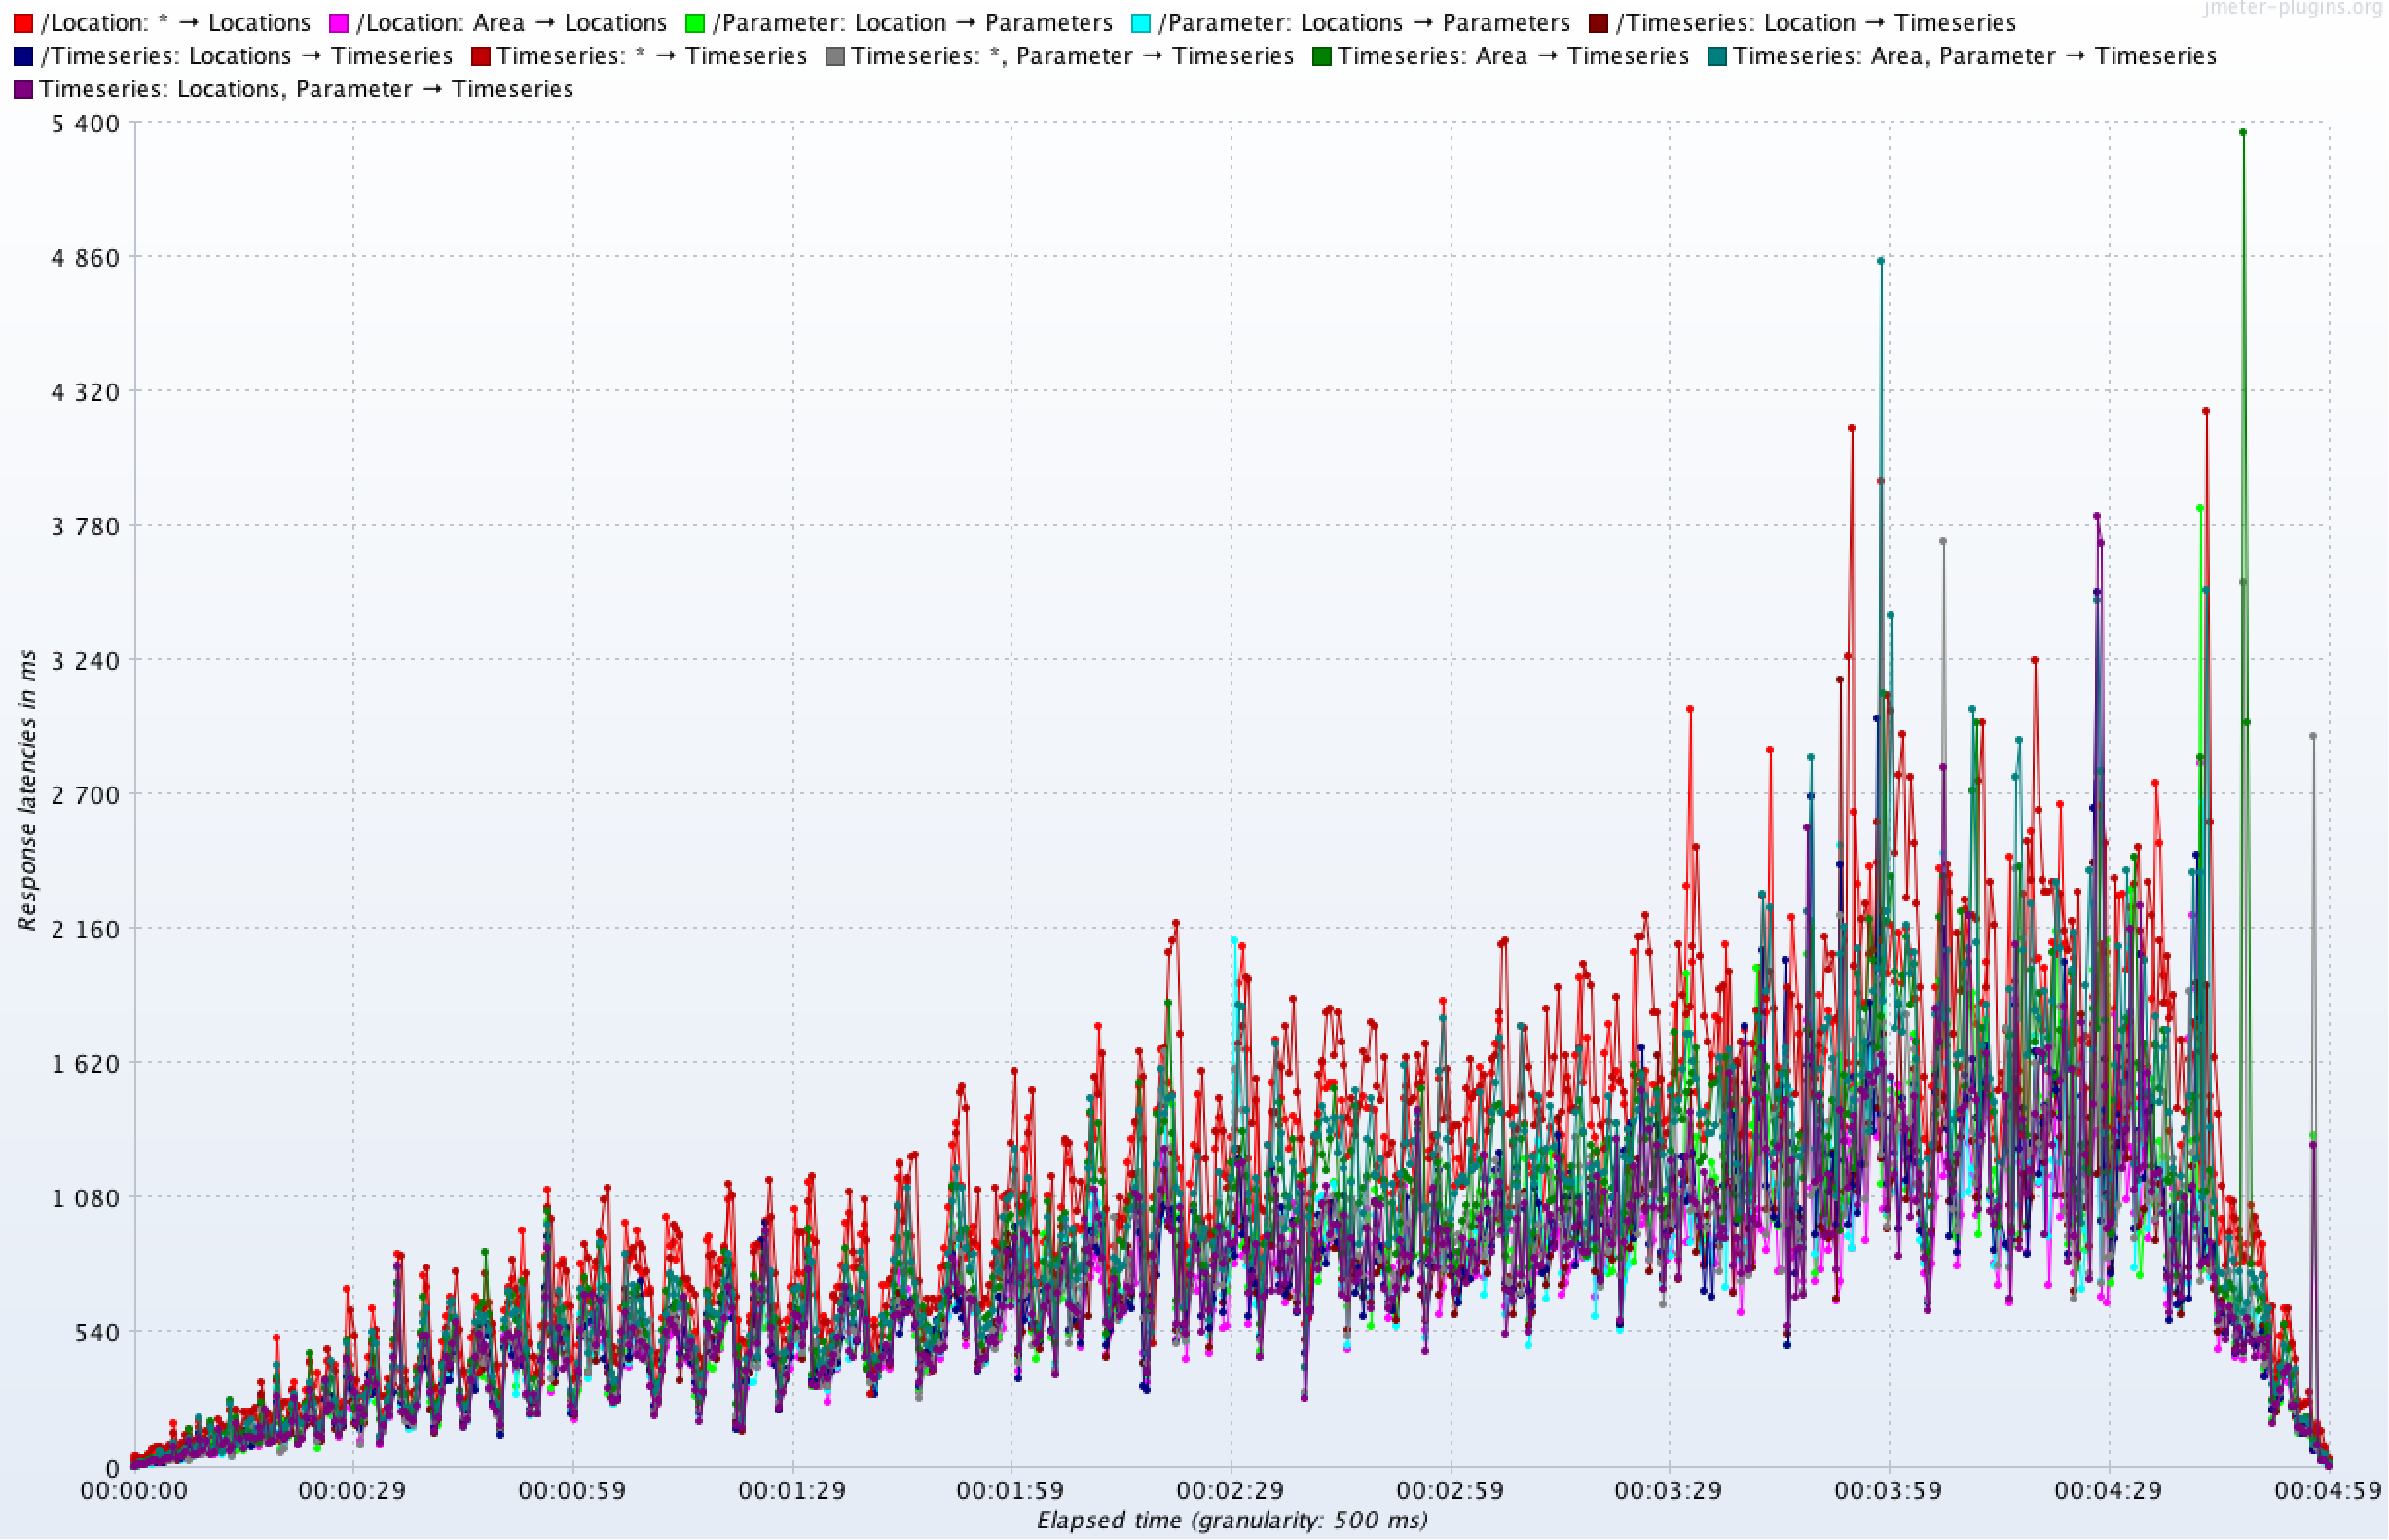
\includegraphics[width=0.8\textwidth]{results/obs/query/obs_query_5m_latency_over_time.png}
    \caption{Load testing query test over 5 minutes - Response Latency over Time}
    \label{fi:test_obs_query_5m_response_latency}
\end{figure}
\ref{fi:test_obs_query_5m_response_latency} shows the response latency over time for the query test plan. When the number of request get higher, the latency also get increased. That means adapter-query is not very much scalable with the current configurations.

\begin{figure}[htp]
    \centering
    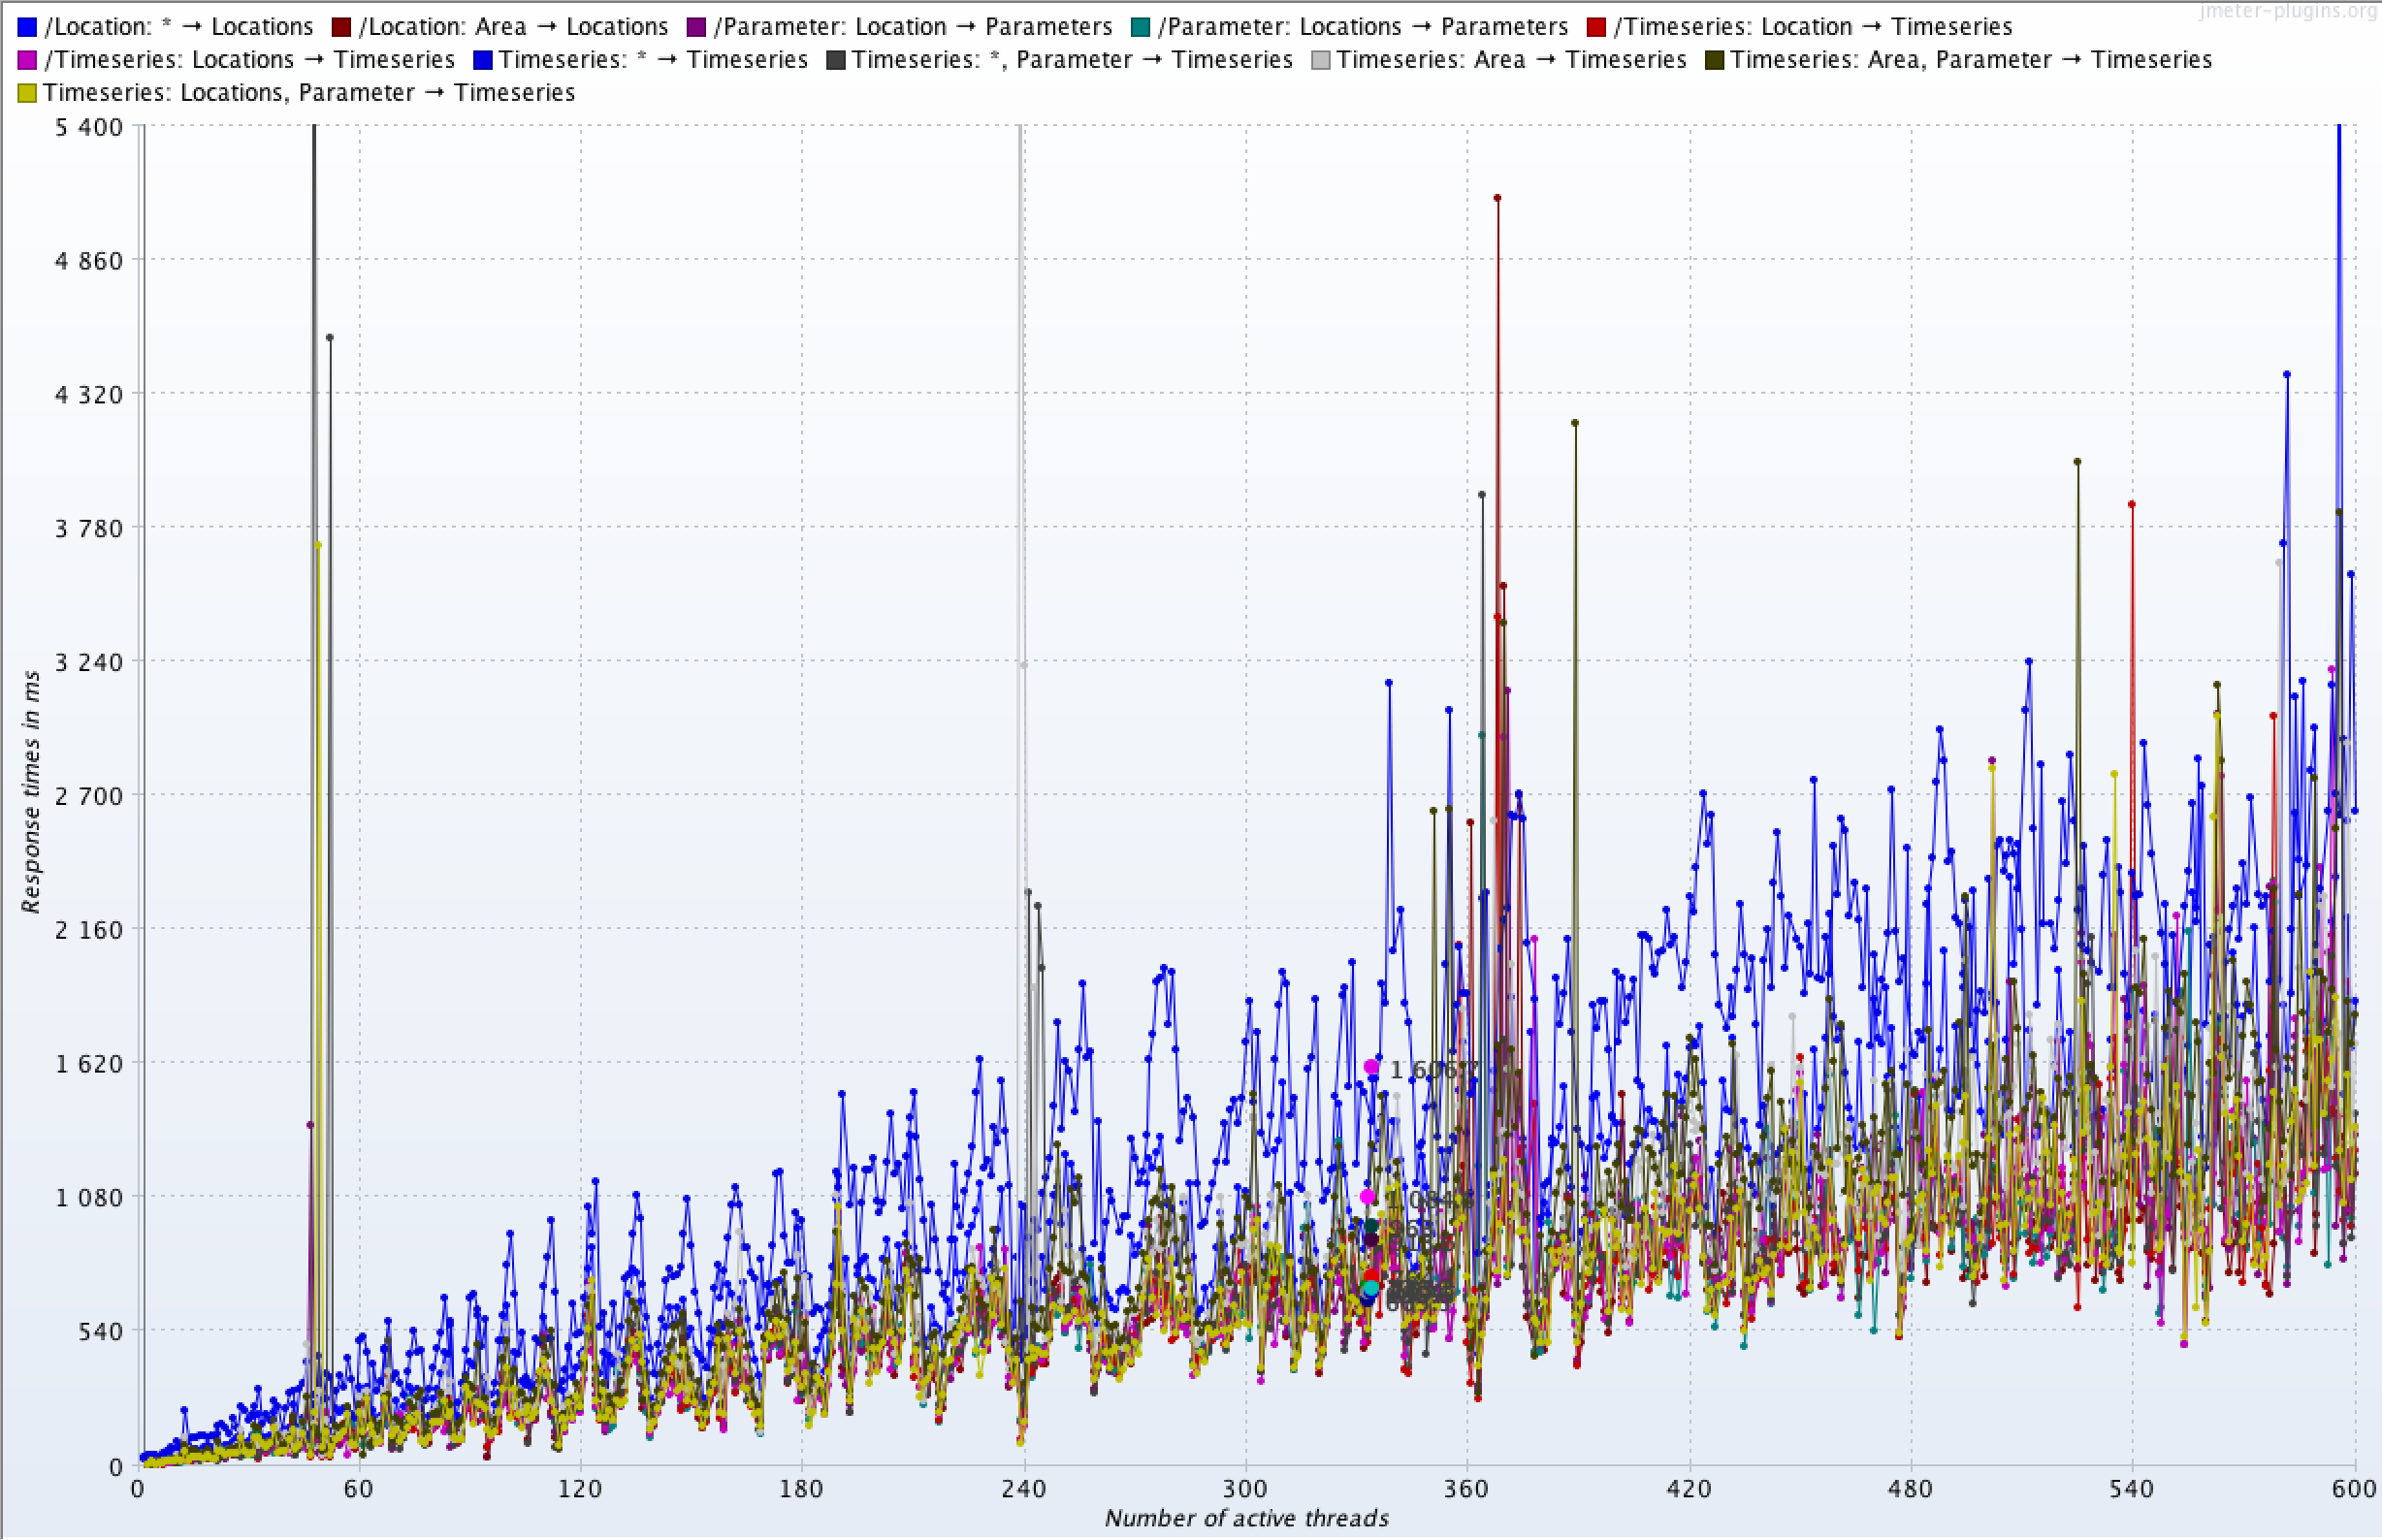
\includegraphics[width=0.8\textwidth]{results/obs/query/obs_query_5m_response_times_vs_threads.png}
    \caption{Load testing query test over 5 minutes - Response Latency Times vs Threads}
    \label{fi:test_obs_query_5m_response_times_vs_threads}
\end{figure}
\ref{fi:test_obs_query_5m_response_times_vs_threads} shows the response latency against number of active threads for the query test plan. When the number of server hits get higher, the latency also get increased. That means adapter-query is not very much scalable with the current configurations.

When ever the timeseries data not found in the adapter-query, it read data from adapter-metadata and index for search over timeseries metadata. This will cause to higher performance with geo timeseries searches. The performance of the \acrshort{mongodb} can further improve with using it features like Replication for high availability, and Sharding for higher throughput.
Those attempts are beyond the scope of \acrshort{wdias} performance test and users can use those to get higher results from the \acrshort{wdias}.
